
\documentclass[11pt]{article}

%% Language and font encodings
\usepackage[english]{babel}
\usepackage[utf8x]{inputenc}
\usepackage[T1]{fontenc}
\usepackage{amsmath}
\usepackage{helvet}
\renewcommand{\familydefault}{\sfdefault}
% Referencing format
%\usepackage[sort, numbers, super, square]{natbib}
\usepackage{breakcites}

%% Sets page size and margins
\usepackage[a4paper,margin=25mm, headheight=13.6pt]{geometry}
\fontsize{11pt}{13pt}

%% Useful packages
\usepackage{amsmath}
\usepackage{xfrac}
\usepackage{graphicx}
\usepackage[colorinlistoftodos]{todonotes}
\usepackage[colorlinks=true, allcolors=blue]{hyperref}
\usepackage{titling}
\usepackage{parskip} %removes indents on new paragraphs
\usepackage[toc,page]{appendix}
\usepackage{chngpage}

\usepackage{csquotes}
\usepackage{tikz-3dplot}
\usetikzlibrary{lindenmayersystems}

\usepackage{pgfplots}
\pgfplotsset{width=10cm,compat=1.9}


\usepackage[ruled, vlined]{algorithm2e}
\usepackage{mathtools}


%Figures
\usepackage{wrapfig}
\usepackage{caption}
\usepackage{subcaption}
\usepackage{chngpage}
\usepackage{float}
\usepackage[capitalise]{cleveref}

%figures to end
% \usepackage[nomarkers,nolists]{endfloat}
% \renewcommand{\efloatseparator}{\mbox{}}

%Colours for notes and shit
\usepackage[colorinlistoftodos]{todonotes}
\usepackage{xcolor}

\usepackage{fancyhdr}
\usepackage{multirow}
\usepackage{rotating}
\usepackage{adjustbox}

\pagestyle{fancy}
\pagestyle{fancy}
\fancyhf{}
\rhead{\thepage}
\lhead{\textit{Contents}}
\renewcommand{\headrulewidth}{0pt}

\definecolor{James}{RGB}{0, 94, 244}

\DeclarePairedDelimiter\abs{\lvert}{\rvert}%
\DeclarePairedDelimiter\norm{\lVert}{\rVert}%

% Swap the definition of \abs* and \norm*, so that \abs
% and \norm resizes the size of the brackets, and the 
% starred version does not.
\makeatletter
\let\oldabs\abs
\def\abs{\@ifstar{\oldabs}{\oldabs*}}
%
\let\oldnorm\norm
\def\norm{\@ifstar{\oldnorm}{\oldnorm*}}
\makeatother

\captionsetup{justification=centering}


\begin{document}
\begin{titlepage}

\vspace*{1cm}

\begin{center}
    \textbf{\LARGE UNIVERSITY OF BRISTOL}
    
    \vspace{3em}
    
    \textbf{\Huge DEPARTMENT OF \\ \vspace{0.5em} ENGINEERING MATHEMATICS}
    
\end{center}
\vspace{3cm}

\center
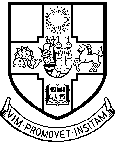
\includegraphics[width=0.18\textwidth]{Images/Misc/bristol_emblem.png}\par\vspace{1cm}

\vspace{2.5cm}

{ \huge \bfseries THE ART OF PERSUASION
}\\

\vspace{3cm}

{ \large \bfseries James Keen (Engineering Mathematics)
}\\

\vspace{1.5cm}

{\large Project thesis submitted in support of the degree of Master of Engineering}

\vspace{0.7cm}

\today

\vspace{0.25em}


\raggedright \textit{Supervisors: Prof. John Lawry, Mr Michael Crosscombe,  Engineering Mathematics}

\end{titlepage}

\pagenumbering{roman}
\begin{abstract}
    
Also a test

\end{abstract}
% \setcounter{tocdepth}{1}     % (Could use this to shorten things further)

\tableofcontents

\newpage
\section*{Table of Notation}
\begin{table}[H]
\begin{tabular}{c|c|l} \hline
Symbol & Type &  Meaning \\ \hline
$S$ & agent & The agent selected as speaker \\
$L$ & agent & The agent selected as listener\\ 
$x$ & agent & An agent drawn randomly from the population \\
$y$ & set of agents & A set of agents selected at random from the population  \\ \hline

$s$ & index & The index of the speaker   \\
$l$ & index & The index of the listener\\
$i$ & index & The index of an agent\\
$j$ & index & The index of a state\\
$t$ & index & The current time step of the system\\  \hline 

$n$ & scalar & The number of possible states of the world \\
$K$ & scalar & The number of agents in a population \\
$t_{max}$ & scalar & The maximum number of iterations \\
$T$ & scalar & The number of iterations for convergence \\
$\eta$ & scalar & The threshold for convergence\\
$\sigma$ & scalar & The standard deviation \\
$\gamma$ & scalar & The threshold on the speakers $[0,1]$\\
$\alpha$ & scalar & The importance of new information an agent receives $[0,1]$ \\
$\epsilon$ & scalar & An arbitrarily small number \\
$\tau$ & scalar & The number of arguments an agent has received \\
$\phi$ & scalar & The rate of acclimatisation \\
$\pi$ & scalar & The probability of receiving a piece of evidence\\
$c$ & scalar & The probability a piece of evidence is accurate \\
$\zeta$ & scalar & The number of arguments used to reconstruct beliefs\\
$\hat{E}^t$ & scalar & Average entropy of the population at time $t$ \\
$\hat{J}^t$ & scalar & Average J-Divergence of the population at time $t$ \\
$\lambda$ & scalar & An eigenvalue of a matrix \\ \hline


$\underline{\underline{\mathbf{P}}}^t$ & matrix & A matrix representing the beliefs of each agent at time $t$ \\
$\underline{\mathbf{P}}^t_i$ & vector & A column vector agent $i$'s beliefs at time $t$\\
$\hat{p}^t_{x,j}$ & scalar & The approximated probability value of $x$'s belief in $H_j$ \\
$p_{i,j}$ & scalar & The probability value agent $i$ holds for state $j$\\
$P_x()$ & function & A function that returns the probability agent $x$ holds for a set of states\\ \hline

$\mathbf{W}$ & set of states & The set of all possible worlds \\
$\mathbf{H}$ & set of states & A set of possible states \\
$H_j$ & state & The $J^\textnormal{th}$ possible state of the world \\
$\mathbf{A}$ & set of states & The set of states that the speaker asserts \\
$\mathbf{A}_\zeta$ & set of states & A set of the last $\zeta$ states an agent has asserted \\
$\underline{\mathbf{A}}$ & vector & A binary vector indicating the presence of a state in $\mathbf{A}$ \\ \hline 


$\underline{\underline{\mathbf{J}}}$ & matrix & The Jacobian matrix \\
$\underline{\underline{\mathbf{M}}}$ & matrix & An arbitrary matrix\\ \hline

$D(c, r)$ & Gershgorin Disc & A Gershgorin Disc centred about $c$ with radius $r$ \\ \hline



\end{tabular}
\end{table}



% \todo[inline]{Tie the ELM in to later stages of the report  }
\newpage

\pagenumbering{arabic}

\pagestyle{fancy}
\fancyhf{}
\fancyhead[CE,CO]{\leftmark}
\fancyfoot[LE,RO]{Page \thepage}
\fancyfoot[RE,LO]{1. INTRODUCTION}
\renewcommand{\headrulewidth}{1pt}
\renewcommand{\footrulewidth}{1pt}

\chapter{Introduction}

The evolution of opinions in multi-agent systems is a well-studied field. In these systems, agents share information in order to reach a consensus. The field of Opinion Dynamics focusses on methods for a single agent to combine information from the population to formulate its own beliefs. However, little attention is paid to the content of the information that is broadcast, with agents often revealing the full and exact nature of their beliefs. Such openness is both a lack of privacy and a lack of precision, as an agent might share more information than is relevant. To mitigate this, it is possible to structure the information that is shared; only the most pertinent material that will persuade an agent to change their opinion to align more closely with the new information will be broadcast.

The provision of a structure to the design of communications between agents also improves a current affliction of Artificial Intelligence. The rationale behind an agent's decision is often unclear~\cite{Doran2017WhatPerspectives}. Hence, it is important to understand the process the agent has undergone to formulate its beliefs, in order to clarify the reason behind its decisions. A structure also improves the understanding of the decision-making process of a population as a whole, such as a swarm of robots that must reach a decision that is best for the group. This paper studies the effects of persuasion on the evolution of opinions in a virtual population~\cite{Harvey2019QuantitativeMarking}. 

Persuasion in human interactions is well studied qualitatively, revealing it to be a multi-faceted phenomenon. One of the most prevalent definitions is as follows:

\begingroup
\addtolength\leftmargini{0.1in}
\begin{quote}
    \textit{Persuasion refers to any change in attitudes that results from exposure to a communication.} \cite{Petty1986CommunicationChange}
\end{quote}
\endgroup


Models are proposed in~\cref{sect:speaker_models} that provide structure to the creation of a communication, and mechanisms for changes in attitude are discussed in~\cref{sect:listener_models}. 

The qualitative features of persuasion are ill-defined quantitatively, making them difficult to incorporate directly into these models. The Elaboration Likelihood Model (ELM) categorises these features into two main ``routes'' for persuasion~\cite{Petty1997ThePsychology}: the Peripheral and the Central Route. The Peripheral Route describes influence that is achieved indirectly, through invoking a positive sentiment that an individual might associate with a notion or object. This method aims to alter a person's attitude subconsciously and often results in only temporary changes in attitude. The Central Route is the more direct approach with arguments and reasons being exchanged without pretence. Due to the temporary and vague nature of the persuasion through the Peripheral Route, it is this Central Route that motivates the work that follows. 

In order to model influence via the Central Route, it is important to understand what variables impact it. For instance, the ELM describes a spectrum of the listener's predisposition to apply significant cognitive effort toward analysing an argument. Those who prefer to dissect new information are most responsive to a strong argument, with few flaws, no matter who presents it. Alternatively, those indisposed to effortful thought surrounding an argument are much more likely to respond positively to the argument if it comes from a source they believe to be expert and reliable. Another impactful factor is the mood of the recipient of an argument; those in a good mood are more likely to accept the argument, while those in a more negative frame of mind are more prone to counter-arguing~\cite{Petty1997ThePsychology}. 

The importance of understanding these routes in the context of this report can be demonstrated with an example. Consider a psychologist and their patient. If the patient were to hold a set of destructive and dangerous beliefs, it is the psychologist's duty to persuade the patient to alter their beliefs so as to improve their health. Equivalently, if an artificial agent were to hold a set of destructive and dangerous beliefs, it is the duty of the designer to persuade the agent to alter its beliefs to be closer to those intended.  Instead of resetting such an agent and destroying its knowledge base, it is plausible that one could persuade the agent to alter its beliefs with a rational argument. 

One of the closest technological approximations to a human mind at present are Deep Neural Networks. Therefore, analogues to human persuasion can be found there. Several prominent technology companies are pursuing deep learning as a method for complex communication techniques, of which persuasion is a key element~\cite{Dulac-Arnold2015DeepSpaces, Lowe2019OnCommunication, Guo2017LearningTexts}. For instance, researchers have investigated the use of SVM's to quantify the persuasive and rhetorical power of speeches by US presidential candidates. The research established differences in the persuasiveness of Democratic and Republican candidates based only on four-sentence chunks of their speeches~\cite{Strapparava2010PredictingDiscourses}. The following examples of persuasive technology are from Facebook, IBM and Google respectively.

Facebook has explored neural networks capable of persuasion in the form of natural language negotiation. The researchers analyse a number of possible factors in successful negotiations, including persuasion~\cite{Lewis2017DealDialogues}. Here, the authors attempt to train a pair of networks to negotiate a deal. Each network was given an inventory of arbitrary objects and values. Their objective was to trade items with one another in order to obtain a particular item. They were trained using a dataset of transcriptions of crowd-sourced interpersonal deal-making. This project failed to create agents proficient enough in the use of natural language to be successful. Not only this, but the agents also learned to deceive their counterparts. They would systematically understate the value of the object they were targeting attempting to persuade their opponent to give them the best possible deal~\cite{Lewis2017DealDialogues}. This was due to the presence of deception in the training data. Similar behaviour can be observed in the field of experimental economics in~\cite{Smith1976ExperimentalTheory}, a seminal paper on market games. Here, the participants were assigned the role of buyer or seller in a continuous double auction and tasked with making a deal. It was found that the buyers would naturally bid lower than their limit price, and the sellers would do the opposite.

The state-of-the-art in persuasive deep learning methods is Project Debater from IBM, which provides a competitive debating engine. Given a topic and a short amount of time, it can generate a compelling narrative in support of the claim it intends to make (see~\cite{Hou2017ArgumentModel, Mass2018WordSpeech} for more detail). The agent's goal is both to persuade the judges and to respond to the opponent in a formal debating style. To achieve this, the agent is trained on a vast corpus of publicly available debates, transcripts and Wikipedia articles. The agent must identify the most salient aspects of a sentence for the claim in question, extract that information, determine its relevance, and then incorporate it into a compelling speech~\cite{Levy2018TowardsSupervision}. The ``convincingness'' of this speech is learned from a dataset of human debates labelled by professional debaters who determine the relative ``convincingness'' of one motion against another~\cite{Habernal2016WhichLSTM}. The authors conclude that this is an effective tool in quantifying the power of an argument and that the errors in the results are likely attributed to ambiguous topics rather than significant flaws in the design of the network. This project also incorporates novel aspects of speech recognition into both the agent's ability to comprehend its opponent's assertions and to rebut them. Whereas previous attempts at sentiment analysis were trained using only text-based transcriptions of public debates, Project Debater extends this to auditory data. This captures the tonality of the speaker so as to better comprehend the claim and sentiment of the argument. The results of this work are preliminary but show that the field of listening comprehension can be incorporated into artificial argumentation and reasoning.


Despite their communicative aptitude, neural networks are vulnerable to targeted adversarial attacks on their decision-making processes. A sufficiently trained network can assign a specific label to a given input. It can also be persuaded to assign a different label if there is a particular adversarial perturbation to that same input. For example, consider a neural network trained to recognise a wide variety of images~\cite{Krizhevsky2012ImageNetNetworks}. \Cref{fig:adversarial_patch} shows an example of such a classifier. Upon receiving an image of a banana, it is the estimation of the network that the image shows a banana. However, when the input is altered, the network changes the label it assigns, incorrectly believing that the image now shows a toaster~\cite{Goodfellow2014ExplainingExamples, Brown2017AdversarialPatch}. The scene-independent nature of this attack highlights a weakness in the decision-making ability of some neural networks. Here, the attackers exploit the network's tendency to focus on the most salient parts of an image and then base its classification heavily on those sections. \Cref{fig:adversarial_patch} shows that the output of the classifier is incorrect when the sticker is added as it recognises the sticker as the most relevant part of the input image. This change of label is an example of persuasion in an adversarial setting. The network changes its attitude, the label, when exposed to a communication, the sticker. It is especially potent as the attack is not dependent on the input, but on the network architecture, shifting the focus of the classifier regardless of the scene it is placed in. 



\begin{figure}[ht]
    \centering
    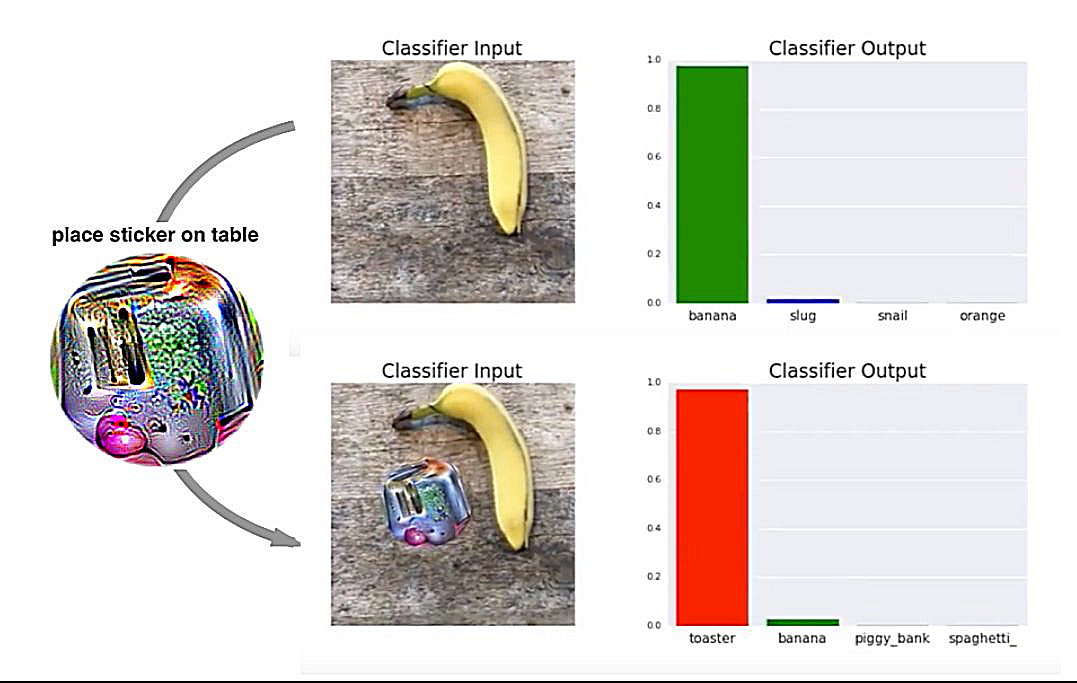
\includegraphics[trim={0, 7mm, 0, 0}, clip, width=0.7\textwidth]{Images/Misc/AdversarialPatches.png}
    \caption{An example of an adversarial patch applied to fool a deep neural network performing object recognition. The network can be seen correctly classifying the object contained within the first image, but when the patch is introduced. The network instead focuses on the patch, incorrectly believing it to be highly relevant in the classification, and thereby ignoring the actual image intended for classification, in this case, a banana~\cite{Brown2017AdversarialPatch}. }
    \label{fig:adversarial_patch}
\end{figure}


There is an extensive literature in the area of opinion dynamics, as it is a useful tool to employ in the analysis of social networks and swarm robotics. Understanding the evolution of ideas and motivations in a population is essential for creating rational and consistent behaviour in groups. A broad description of rationality dictates that an agent must be autonomous, sociable, proactive and reactive~\cite{Genesereth1994SoftwareAgents, Castelfranchi1995GuaranteesArchitecture}. Under these tenets, the agents adhere to a set of simple rules and work cohesively toward the collective goal of the group. This is accomplished without central oversight producing results more complex than any agent could create alone~\cite{Rawls1971AJustice}. A requirement for this is that the majority of the population agrees on the best procedure to follow~\cite{Baronchelli2018ThePrimer}. A unanimous agreement of this nature is referred to as global consensus while an agreement within a subset of the population is referred to as local consensus.


The work of~\cite{Parker2009CooperativeProblem} gives an example of the above, describing a population of agents acting without a central authority. This creates a robust population; they are sufficiently autonomous so as not to be incapacitated should a central node fail. The agents must reach a global consensus in order to achieve their goals. In this example, the population must agree on the location of a nest site. Inspiration for this was drawn from naturally occurring swarms of ant and bee colonies~\cite{Pratt2005BehavioralCurvispinosus, List2009IndependenceSwarms}. In~\cite{Parker2009CooperativeProblem}, the agents follow a set of rules for sharing and discovering new information. This enables them to influence one another to adopt a new set of attitudes that best suit the needs of the colony. This change in attitude demonstrates the importance of persuasion in this population, as defined by~\cite{Petty1986CommunicationChange}. It suits the colony to collectively pursue one single desired outcome rather than dividing their resources in disparate pursuits of multiple unrelated goals. In short, it is better to work in concert toward a goal than in discord, even if the ultimate goal is potentially sub-optimal. This is only made possible through effective affective communication of opinions between the agents, though it can likely be refined. 

The opinion of a single agent can be mathematised using aspects of uncertainty modelling, facilitating the analysis of the evolution of its beliefs~\cite{Wooldridge1995IntelligentPractice}. This requires assumptions such as the Closed World Assumption (CWA), which places a finite limit on the number of possible states that could be true, allowing agents to assign a probability value for each of them~\cite{Jsang2001APROBABILITIES}. For illustrative purposes, consider a world containing $3$ possible states. This can be depicted in two ways. Firstly, consider \cref{fig:hesse}. This diagram shows all the possible subsets of this $3$-dimensional world. The topmost set contains all the possible states of the world and so can be defined as $\mathbf{W} = \{ H_1, H_2, H_3\}$. 

\begin{figure}[H]
    \centering
    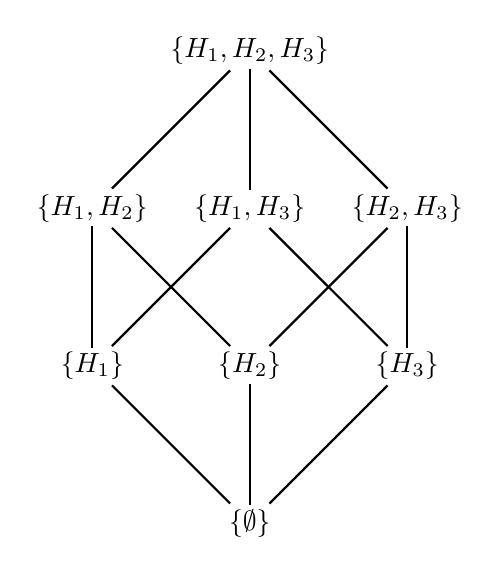
\begin{tikzpicture}
    % First, locate each of the nodes and name them
        \node (top) at (0,0) {$\{H_1, H_2, H_3\}$};
        \node (left) at (-2, -2) {$\{H_1, H_2\}$};
        \node (center) at (0, -2) {$\{H_1, H_3\}$};
        \node (right) at (2, -2) {$\{H_2, H_3\}$};
        \node (one) at (-2, -4) {$\{H_1\}$};
        \node (two) at (0, -4) {$\{H_2\}$};
        \node (three) at (2, -4) {$\{H_3\}$};
        \node (empty) at (0, -6) {$\{\emptyset \}$};

    % Now draw the lines:
        \draw [thick, shorten <=-2pt, shorten >=-2pt] (top) -- (left);
        \draw [thick, shorten <=-2pt, shorten >=-2pt] (top) -- (center);
        \draw [thick, shorten <=-2pt, shorten >=-2pt] (top) -- (right);
        \draw [thick, shorten <=-2pt, shorten >=-2pt] (left) -- (one);
        \draw [thick, shorten <=-2pt, shorten >=-2pt] (left) -- (two);
        \draw [thick, shorten <=-2pt, shorten >=-2pt] (center) -- (one);
        \draw [thick, shorten <=-2pt, shorten >=-2pt] (center) -- (three);
        \draw [thick, shorten <=-2pt, shorten >=-2pt] (right) -- (two);
        \draw [thick, shorten <=-2pt, shorten >=-2pt] (right) -- (three);
        \draw [thick, shorten <=-2pt, shorten >=-2pt] (one) -- (empty);
        \draw [thick, shorten <=-2pt, shorten >=-2pt] (two) -- (empty);
        \draw [thick, shorten <=-2pt, shorten >=-2pt] (three) -- (empty);
    \end{tikzpicture}   
    \caption{A Hasse Diagram for a world with 3 possible states.}
    \label{fig:hesse}
\end{figure}


A probability value in the interval $[0, 1]$ can be assigned to each possible state of the world such that $P(\mathbf{W}) = 1$, forming the opinion of a single agent in the population. It has been shown that human ability to reason under uncertainty seems to follow a probabilistic framework~\cite{Costello2014SurprisinglyJudgment}. Experiments have shown that the participants in the test followed Bayes rule, though corrupted by some noise. This assertion that people take a Bayesian approach has been contested, though the assertion that humans follow a probabilistic reasoning framework is supported~\cite{Douven2018CanAway}. This allows the exchange and evolution of beliefs to be modelled mathematically. 

In the field of opinion dynamics, there are two primary approaches to communication in multi-agent populations. In both, an individual agent $x$ and a subset of the population $y$ are selected at random. $x$ then queries $y$ and receives their entire set of beliefs in response. It is assumed that the population aims to confer and collectively reach a conclusion that is most beneficial to the group as a whole~\cite{Rawls1971AJustice}. The first approach describes various methods for pooling the responses together in order to update $x$'s own beliefs~\cite{Degroot1974ReachingConsensus}. Multiple different functions have been proposed for this, each producing slight variations in the way in which the population converges to a single shared belief~\cite{Lee2018CombiningConsensus}. This pooling aims to make use of the ``wisdom of the crowd'' effect~\cite{Golub2010NaiveCrowds}. This refers to the belief that the more people involved in making a judgement, the more information is available, and so the more accurate the decision will be. However, there are those that argue that the opposite must also be true: the more people present, the more misinformation is available in the decision-making process, thus drowning out the voices of those who may be most accurate~\cite{Dalkey1963AnExperts}. There is experimental evidence in support of the ``wisdom of the crowd'' and decision-making techniques based on it, such as the Delphi Method. This is a technique employed in order to obtain the best verdict from a panel of experts~\cite{Dalkey1963AnExperts}. The method begins with the panellists completing a questionnaire in isolation without communicating with one another. These are then summarised and shown to each member of the group, who are invited to update their responses. This process is repeated until a predetermined condition is met, and shows that this combination of expert opinions often converges to a single clear idea. 

The second approach to the amalgamation of opinions is for $x$ to simplify the combination process, taking an average of the other agents' beliefs weighted by a parameter representing the population's view of their reliability~\cite{Hegselmann2002OpinionSimulation}. This reliability parameter can lend disproportionate influence to a small number of agents, making them dominant factors in the decision-making process. The reverse is also true, with some agents' opinions being disregarded as they are deemed unreliable. The model can be extended to include an element of $x$'s past beliefs, so that they are not lost when updated, for example, in the Friedkin Johnsen (FJ) model~\cite{Friedkin1999SocialChange}. The FJ model takes a linear combination of $x$'s previous beliefs and the weighted average of the population's beliefs, forming $x$'s updated beliefs. This method has also been trialled on humans~\cite{Friedkin2011APower}. Groups of four students were placed in separate rooms and asked to reach a decision as a group within 20 minutes. The only means of communication was a phone in each room, that could not connect to more than one person at a time. These experiments demonstrated that, generally, a single member of the group emerged as the most influential in reaching a collective decision. 

These models are advantageous because the rationale behind the decision made by the agents is interpretable by humans. However, the models can still be improved, as each agent in $y$ broadcasts more information that may be relevant. The complexity in these models is in the behaviour of $x$ upon receipt of new information from $y$. 


\fancyfoot[RE,LO]{\rightmark}
\section{Aims and Motivation}

This project aims to explore the effects of including aspects of persuasion into communication in multi-agent systems. It is important that the population be able to converge to a unanimous agreement in a single shared belief. Without such a consensus, the agents are unable to achieve their full potential and may fail to reach their intended goal. A secondary aim of this work is to provide a structure to the evolution of beliefs in artificial populations. With such a structure, it is possible to more easily explain the rationale behind an agent's communication, and interpret the opinion dynamics of the system. 



In this report, we adopt a simple probabilistic model of beliefs and a speaker-listener model for communication. One agent is selected at random to broadcast a persuasive argument and another is chosen as the listener that must react to the argument at each iteration. \Cref{sect:method} outlines the experimental set up for the models that are described in \cref{sect:speaker_models} and ~\cref{sect:listener_models}. \Cref{sect:analysis} discusses the results found before suggesting a number of extensions to the experimental setup that aim to more closely mimic human behaviours, incorporating aspects of persuasion. This work is concluded with a discussion of the main results and a number of avenues for further work. 










\chapter{Method}\label{sect:method}


\fancyfoot[RE,LO]{2. METHOD}

\Cref{fig:hesse} depicts the powerset of all possible worlds in a $3$-dimensional system. In the models that follow, an agent's opinion is given by its distribution of probabilities over each of these possible worlds, shown as singleton sets in the diagram. Hence, the set of beliefs held by the $i^\textnormal{th}$ agent can be represented by the vector

\begin{center}
$ \underline{\mathbf{P}}^t_i = \begin{bmatrix}
    p_{i, 1}\\
    p_{i, 2}\\
    p_{i, 3}
\end{bmatrix}$,
\end{center}

where $p_{i,j}$ is the probability value that the $i^\textnormal{th}$ agent has placed in state $\{H_j\}$. By the axiom $P(\mathbf{W}) = 1$, the vector $\underline{\mathbf{P}}^t_i$ must also sum to $1$. This allows us to form a right-stochastic matrix\footnote{A right stochastic matrix is defined as a square, non-negative matrix for which the rows sum to $1$~\cite{Gagniuc2017MarkovExperimentation}.} representing the collective beliefs of $K$ agents over $n$ states of the world at time $t$,

\begin{center}
$\underline{\underline{\mathbf{P}}}^t = \begin{bmatrix}
    p_{1, 1} & p_{1, 2} & p_{1, 3} & \dots  & p_{1, n} \\
    p_{2, 1} & p_{2, 2} & p_{2, 3} & \dots  & p_{2, n} \\
    \vdots & \vdots & \vdots & \ddots & \vdots \\
    p_{K, 1} & p_{K, 2} & p_{K, 3} & \dots  & p_{K, n}
\end{bmatrix}$.
\end{center}

Each of the $K$ agents is initialised with $n$ distinct beliefs computed using \cref{alg:initialise}. In a $3$-dimensional case, agents' beliefs can be represented as a point on the blue surface shown in~\cref{fig:3d-simplex}, referred to as a simplex. This surface can be projected down to a $2$-dimensional plot, shown in~\cref{fig:2d-simplex}, referred to as a Barycenter plot. In this plot, an agent in the corner of the triangle is described as being certain, extremist, or having a strong belief in a single hypothesis. Conversely, an agent with uncertain or weak beliefs holds an approximately uniform distribution and so is found in the central region of Barycentric space.

\begin{algorithm}[H]
\SetAlgoLined
\KwResult{Initialisation of the beliefs of $K$ agents }
 \While{$i < K$}{
  $d \gets drawRandomNumbers(n-1)$\;
  $d \gets sort(d)$\;
  $prepend(0, d); append(1,d)$\;
  $beliefs \gets consecutiveElementwiseDifference(d)$;  \hspace{1em} \textit{$\triangleright$ returns list $(j+1)^\textnormal{th}$ - $j^\textnormal{th}$ values}\\
  $i++$\;
 }
 \caption{Agent Initialisation}
 \label{alg:initialise}
\end{algorithm}












\begin{figure}[H]
\begin{minipage}[ht]{0.45\textwidth}
    \centering
    \resizebox{\linewidth}{0.74\linewidth}{
   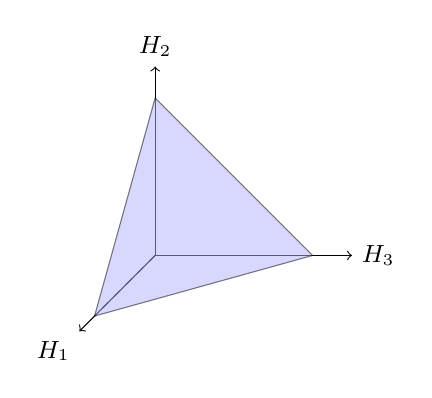
\begin{tikzpicture}[line join = round, line cap = round]
\coordinate [] (A) at (2,0,0);
\coordinate [] (B) at (0,0,2);
\coordinate [] (C) at (0,2,0);
\coordinate [] (D) at (0,0,0);

\draw[->] (0,0) -- (2.5,0,0) node[right] {\small $H_3$};
\draw[->] (0,0) -- (0,2.4,0) node[above] {\small $H_2$};
\draw[->] (0,0) -- (0,0,2.5) node[below left] {\small $H_1$};
\foreach \i in {A,B,C,D}
    \draw[dashed] (0,0)--(\i);
\draw[-, fill=blue!30, opacity=.5] (A)--(B)--(C)--cycle;
\end{tikzpicture} }
\subcaption{$3$-dimensional simplex}\label{fig:3d-simplex}
\end{minipage}
\hfill
  \begin{minipage}[ht]{0.45\textwidth}
    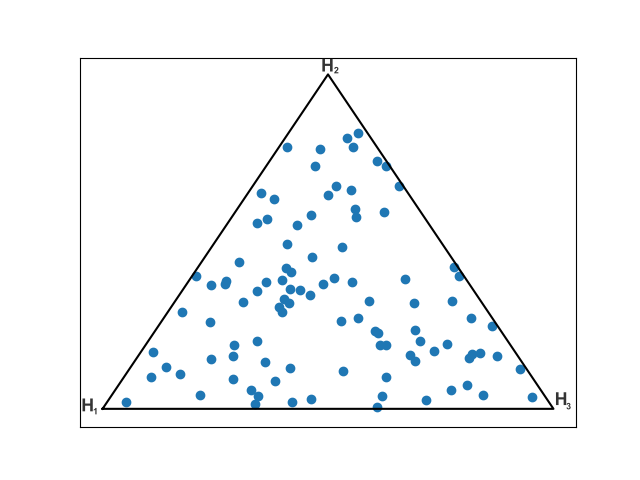
\includegraphics[width=\textwidth]{Images/Figures/Barycenter/ExampleBarycentre.png}
    \subcaption{$2$-dimensional projection}\label{fig:2d-simplex}
 \end{minipage}
\caption{An example of a $3$-dimensional simplex over a world with $3$ possible states, projected down to $2$-dimensions, referred to as a Barycenter plot. } 
\end{figure}

Once the population is initialised, the communication protocols between agents must be defined, requiring a number of simplifications. One such simplification comes from Parker and Zhang, who describe a characteristic of their model which they name the ``well-stirred'' assumption. This assumes that the population is sufficiently mixed together that it is acceptable to select agents at random to communicate. The assumption can be thought of in a similar way to the social lattice described in~\cite{Deffuant2000MixingAgents}, though instead of a simple square lattice, the network is fully connected with communicating pairs selected at random. In \cref{fig:simple_interaction}, two agents are drawn randomly from the population, one to be the speaker, one to be the listener. This model is based on a special case of the signalling games introduced by~\cite{Lewis2002Convention:Study}. This work describes a communicator that acts in its best interests to convey a message that reflects a state of the world that it perceives to be true. The communicator then broadcasts its message to an audience who react to the information they receive. In our case, the audience is one agent, the listener, as shown in~\cref{fig:simple_interaction}. The communication created by the speaker is an argument it hopes will persuade the listener to update its beliefs to more closely align with the speaker's. 

 \begin{figure}[H]
 	\centering
 	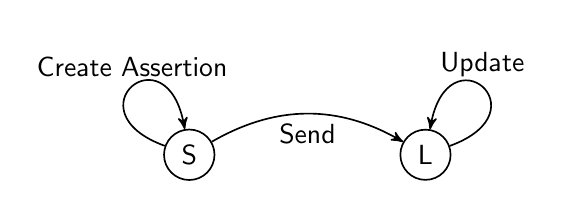
\begin{tikzpicture}[
    ->,
    >=stealth',
    auto,
    semithick,
    node distance=3cm,
    state/.style={
        circle,
        draw,
    },
]
    \begin{scope}[
        every node/.append style={
            state,
        },
    ]
        \node (x0)                     {S};
        \node (x3) [right of=x0] {L};
    \end{scope}
    
    \path
    (x0) edge [loop above, looseness=10, in=100, out=160] node        {Create Assertion}  (x0)
         edge [bend left]                                 node [swap] {Send}              (x3)
    (x3) edge [loop above, looseness=10, in=80, out=20]   node        {Update}            (x3);
\end{tikzpicture}

 	\caption{Simple model of the interaction between two agents. \textit{S} is randomly selected each iteration as the speaker and \textit{L} is randomly selected each iteration as the listener. \textit{S} creates an argument that it transmits to \textit{L}. \textit{L} may then update its own beliefs according to the argument it receives from \textit{S}.}
 	\label{fig:simple_interaction}
 \end{figure}
 
Initially, it is assumed that the speaker is aware of the listener's opinions prior to making an assertion, as well as how the listener will react upon hearing it. \cref{alg:method} is run until either the maximum number of iterations is reached or the system can be said to have converged, as defined in~\cref{eq:convergence}. This is clearly a greatly simplified interaction, and is therefore not equivalent to any human conversation, no matter how simplistic. However, it serves as an approximate model, allowing the behaviour of the population to be studied in a framework that is explainable. 


\begin{algorithm}[H]
\SetAlgoLined
\KwResult{Simulation of agent based communication }
 initialisation\;
 \While{$t < t_{max}$}{
  selectSpeaker\;
  selectListener\;
  speakerConstructArgument\;
  listenerReactToArgument\;
  \eIf{converged}{
   break\;
   }{
   t++\;
  }
 }
 \caption{Method}
 \label{alg:method}
\end{algorithm}

There are several useful metrics for describing the dynamics of this system. The average entropy of the population as a whole gives the level to which the agents have become certain in a single state~\cite{Shannon1948ACommunication}. This is defined as

\begin{equation}\label{eq:shannon_entropy}
    \hat{E}^t = \frac{1}{K} \sum_i^K - \underline{\mathbf{P}}^t_i \cdot \log ( \underline{\mathbf{P}}^t_i).
\end{equation}

The system is said to have converged when the entropy has not changed by more than $\eta $ for $T$ iterations, expressed as 

\begin{equation}\label{eq:convergence}
    \Delta \hat{E}^T = \abs{ \hat{E}^t -  \hat{E}^{t+T}}  \leq \eta. 
\end{equation}

However, entropy only highlights whether the agents hold strong beliefs, not that they agree on those beliefs. Hence, the J-Divergence is used as a symmetric version of KL-Divergence, to determine the average distance between all pairs of agents $(i,k)$ in probability space~\cite{Johnson2001SymmetrizingDistance}. It is defined as

\begin{equation}
    \hat{J}^{t} = \frac{1}{K} \sum_k^K \frac{1}{K} \sum_i^K  \frac{1}{2} \left( \underline{\mathbf{P}}^t_i \log \left( \frac{ \frac{1}{2} (\underline{\mathbf{P}}^t_i + \underline{\mathbf{P}}^t_k) }{\underline{\mathbf{P}}^t_i} \right) +  \underline{\mathbf{P}}^t_k \log \left( \frac{ \frac{1}{2} (\underline{\mathbf{P}}^t_i + \underline{\mathbf{P}}^t_k) }{\underline{\mathbf{P}}^t_k} \right) \right).
\end{equation}

The two aspects of~\cref{fig:simple_interaction} are the creation of the speaker's assertion and the response of the listener. For the former, four models are proposed ranging from simply broadcasting the speaker's beliefs to tailoring the argument to the listener. For the latter, four models are defined describing different behaviours the listeners can adopt. These include the listener reacting passively, with discernment, or with steadily less and less importance placed on new information as time passes.








\section{Speaker behaviours in collective decision-making} \label{sect:speaker_models}

In the design of the models that follow, it is important to consider the ethics behind Captology, the study of persuasive technologies~\cite{Atkinson2006Captology:Review}. For instance, it is clearly unethical for a persuasive technology to incite an individual to violence. The work of \cite{Berdichievsky1999TowardsTechnology} provides a preliminary set of rules that such a technology should abide by. Chief among them is the so-called ``Golden Rule'', stating that ``The creators of a persuasive technology should never seek to persuade a person or persons of something they themselves would not consent to be persuaded to do''. Further rules outline the requirement that the technology does not deceive in order to achieve its attempt at persuasion~\cite{Calvo2014TheComputing}. The following models describe agents that are only capable of creating an argument that they themselves believe to be credible, with the exception of the final model. This model is a ``dark side'' example, designed to explore the effects of removing this inhibition~\cite{Berdichievsky1999TowardsTechnology}.

\subsection*{Open Model}

The assertion that the speaker selects should reflect the underlying set of beliefs in the agent and also produce the desired reaction from the listener~\cite{Lewis2002Convention:Study}. The goal of the speaker is to align the listener's beliefs more closely with its own. The previous approaches to this problem have been to transmit a complete representation of the speaker's set of beliefs at time $t$~\cite{Degroot1974ReachingConsensus, Lee2018CombiningConsensus, Friedkin1999SocialChange, Hegselmann2002OpinionSimulation}. This requires the speaker to be totally open about the nature of its beliefs, broadcasting  $\underline{\mathbf{P}}_{s}^t$, where $s$ is the index of the speaker. Here, the assertion takes the form of an $n$-dimensional vector of values in the interval $[0,1]$ that sum to $1$, given by

\begin{center}
\begin{equation}
\underline{\mathbf{P}}^t_s = \begin{bmatrix} p_{s, 1}\\ p_{s, 2}\\ \vdots \\ p_{s, n} \end{bmatrix}.
\end{equation}
\end{center}


The dynamics of the Open model are explored in~\cref{sect:analysis}. One benefit of this model is that it is highly transparent, allowing an observer to precisely track the population's beliefs as they evolve. 


\subsection*{Bottom Up Model}

The models hereafter are less revealing, allowing the speaker to assert a set of states, rather than a probability vector over all of them. This approach mirrors the finding that, in humans, a person often prefers to receive absolute information, instead of the uncertainties involved. For instance, when a patient receives a serious diagnosis, they are likely to prefer hearing an unambiguous statement, rather than the probability that it is true~\cite{Fischhoff1982LayRisk}. Consider \cref{fig:hesse}. An agent practising the Bottom Up approach, as intimated, defines its assertion by considering the bottom layer of the Hasse diagram. Any state $H_j$ for which the speaker $s$ has sufficiently high probability $p_{i,j}$ is included in the assertion, similar to the so-called Principal Principle~\cite{IgorDouven2006AssertionCredibility, Lewis1980AChance}. More formally, 

\begin{equation}
    \mathbf{A} = \{ H_j: p_{i,j} > \gamma  \},
\end{equation}

where $H_j$ represents the $j^{\textnormal{th}}$ state of the world and $\gamma$ is a threshold in the interval $[0,1]$ consistent across all agents. Practically, $\mathbf{A}$ can be viewed as a $1 \times n$ binary membership vector given by applying an indicator function to the asserted set, and in this vector form, is notated as $\underline{\mathbf{A}}$. This model shields the internal beliefs of the speaker while only allowing it to put forward assertions it believes to be true above a certain level. It should be noted, however, that for values of $\gamma > 0.5$, the speaker can only assert a singleton set containing one element. This is the most precise assertion that can be made. Furthermore, the assertion of both $\emptyset$ and $\mathbf{W}$ reveal nothing, as these are equivalent to arguing ``I believe nothing to be true'' or ``I believe the true state to be possible'', neither of which contribute anything new to a discussion. 

An interesting feature of this model is that, for $\gamma > \frac{1}{n}$, a region of probability space exists in which it is not possible for an agent to create a meaningful assertion. Take, for example, $\gamma = 0.4, n=3$. It is possible that there exists an agent at time $t$ that is selected as speaker with a set of beliefs

\begin{center}
    
$\underline{\mathbf{P}}^t_s = \begin{bmatrix}
    0.35\\
    0.35\\
    0.3
\end{bmatrix}.$
\end{center}

In this particular example, it is impossible for the agent to assert anything, as no $p_{s,j}$ is greater than $\gamma$. This can result in distributions of the population where the agents are incapable of speech, creating a mute population at a steady state by definition. 

\subsection*{Top Down Model}

As opposed to the Bottom Up model, this method constructs  assertions starting from the top of~\cref{fig:hesse}. Here, the agent iteratively eliminates elements of the set $\mathbf{W} = \{H_1, H_2, \dots, H_n  \}$ for which the probability value $p_{s,j}$ is lowest. The agent will compute its own probability in the argument $\mathbf{A}$ by summing the probabilities of the states within the set. If this sum is above a threshold $\gamma$ then the agent will broadcast the argument. Otherwise, it will remove the element associated with the minimum probability in its set of beliefs. \Cref{alg:TD} outlines the methodology in more detail. This approach can be written as


\begin{equation}
    \mathbf{A} = \{ H_j: P(\mathbf{H}) > \gamma  \},
\end{equation}

where $\gamma$ is again a threshold kept consistent across all agents, $H_j$ is the $j^{\textnormal{th}}$ possible state of the world, and $P(\mathbf{H})$ is the probability of the set of states $\mathbf{H}$, where $\mathbf{H}$ is obtained by the method described in~\cref{alg:TD}.

This method aims to reduce the assertion $\mathbf{A}$ to the most precise set of possible states that still seems plausible to the speaker. Therefore, this method only allows the speaker to make an assertion that it believes to be true. However, it is important to note that the significance of $\gamma$ differs between the Bottom Up and the Top Down models. In the former, it is a threshold that only applies to individual states, whereas in the latter, it relates to sets of states. Consequentially, the two models cannot be compared directly for the same value of $\gamma$. \\

\begin{algorithm}[H]
\SetAlgoLined
\KwResult{Assertion $\mathbf{A}$ }
 \While{$j < n$}{
  $H_{min} \gets min(\underline{\mathbf{P}}_s)$\;
  $\mathbf{H} \gets \mathbf{H} \setminus \{H_{min}\}$\;
  $p \gets P(\mathbf{H})$\;
  \eIf{$p \leq \gamma$}{
   $\mathbf{A} \gets \mathbf{H}$\;
   return $\mathbf{A}$\;
   }{
   j++\;
  }
 }
 return $\mathbf{H}$\;
 \caption{Top Down Model} \label{alg:TD}
\end{algorithm}

\subsection*{Optimised Model}

The speakers in previous models have failed to make use of one valuable piece of information. They do not consider the beliefs of the listener in the construction of their assertions. This is addressed in the Optimised model. 

It is assumed that all agents have perfect information; they know the beliefs of every other agent as well as how they might react to hearing new pieces of information. It is therefore feasible for the speaker to devise the best possible argument for each and every listener. The best outcome for the speaker is that the listener updates their set of beliefs to be as close to the speaker's as possible, thus minimising the J-Divergence between the two. This can be posed as the following unconstrained Integer Programming optimisation problem, 

\begin{equation}
    minimise \hspace{1.2em} z = \frac{1}{2} \left( \underline{\mathbf{P}}^t_s \log \left( \frac{ \frac{1}{2} (\underline{\mathbf{P}}^t_s + \underline{\mathbf{P}}^{t+1}_l(\mathbf{A})) }{\underline{\mathbf{P}}^t_s} \right) +  \underline{\mathbf{P}}^{t+1}_l(\mathbf{A}) \log \left( \frac{ \frac{1}{2} (\underline{\mathbf{P}}^t_s + \underline{\mathbf{P}}^{t+1}_l(\mathbf{A})) }{\underline{\mathbf{P}}^{t+1}_l(\mathbf{A})} \right)     \right),
\end{equation}

where $\underline{ \mathbf{P}}_s$ and $\underline{\mathbf{P}}_l$ are the speaker's and listener's beliefs respectively, and $\underline{\mathbf{P}}_l^{t+1}$ is a function of the argument $\mathbf{A}$ that the speaker broadcasts. This system empowers the speaker to make any argument it needs to in order to convince the listener, regardless of the speaker's own opinions. It would be simple to introduce an integrity constraint, restricting the speaker to only assert states that it itself believes. However, it is also interesting to investigate the effects of allowing an agent total freedom in its choice of argument. This is a ``dark side'' experiment, designed to elucidate an ethically questionable option~\cite{Berdichievsky1999TowardsTechnology}. 



\subsection{Audience behaviours in the collective decision-making process} \label{sect:listener_models}

\subsection*{Simple Listener Model}
Having addressed multiple ways for the speaker to construct an argument, it is imperative to define the strategies that listener agents may employ to update their attitudes. Drawing inspiration from the Friedkin and Johnsen model~\cite{Friedkin1999SocialChange}, we define an update rule that maintains an element of the agents previous beliefs as well as assimilating the new information. 

The equation we will use shall be


\lhead{\textit{Listener Models}}
\begin{equation} \label{eq:BU_update_rule}
    \mathbf{P}^{t+1}_L = \alpha \cdot \mathbf{P}^{t}_L + (1 - \alpha) \cdot  \frac{\mathbf{A} \odot \mathbf{P}^t_L}{\mathbf{A} \cdot \mathbf{P}^t_L}
\end{equation}

where $\alpha$ is a parameter on the interval $[0, 1]$ that governs the susceptibility of an agent to new information~\cite{Hegselmann2002Opinion}. In Hegselmann's work this parameter differs depending upon how reliable the listener believes the other agent to be, while, here, it is constant across all agents. Finally, $\odot$ denotes the elementwise or Haramaard product~\cite{Johnson1990MatrixApplications}. The last component of this equation serves to condition the speaker's argument $\mathbf{A}$  on the listener's original beliefs and then renormalise this such that the agent's probability distribution remains valid by summing to $1$. Any agent whose set of beliefs loses this property is described as incoherent and withdrawn from the population~\cite{Lee2018CombiningConsensus}. Furthermore, it is important to manage the listeners use of this update equation as, in the case where the cardinality of the set $\mathbf{A}$, $|\mathbf{A}| = 0$ \cref{eq:BU_update_rule} is undefined. In this case, the listener simply will not update.  

It should be noted that the Open Model represents a special case. The above equation is tailored toward arguments of binary vectors so if the Open Model is applied the equation becomes 

\begin{equation} 
    \mathbf{P}^{t+1}_L = \alpha \cdot \mathbf{P}^{t}_L + (1 - \alpha) \cdot \mathbf{A} 
\end{equation}


\subsection*{Discerning Model}

The previous model deprives the listener agent of the ability to disregard any information it receives; it will always update its beliefs based on new information. In order to address this, the model requires that when the listener reverses the process used to create the argument on its own beliefs, the same condition must be met. This is only possible in the Bottom Up and Top Down models as they involve a specified criterion that the argument must meet to be transmitted. Consider the following example for illustration. 

Let the speaker broadcast \hspace{10em}

\begin{minipage}[ht]{0.45\textwidth}
\begin{center}
$\mathbf{A} = \begin{bmatrix}
    1\\
    0\\
    1
\end{bmatrix}$
\end{center}
\end{minipage}
and let
\begin{minipage}[ht]{0.45\textwidth} 
$P^t_L = \begin{bmatrix}
    0.6\\
    0.15\\
    0.25
\end{bmatrix}$
\end{minipage}

In the case that this argument is constructed with the Bottom Up method with a threshold $\gamma = 0.4$, the listener compares the argument with its own beliefs. It finds that $p_1 > \gamma$ passing the requirement, $p_2$ is not asserted so is not considered, and finally $p_3 < \gamma$. Since the assertion of $H_3$ seems unlikely to the agent, it rejects the assertion outright, refusing to update. Similarly, if the argument is created with the Top Down model with a threshold $\gamma = 0.8$, then the listener takes the dot product of $\mathbf{A}$ and $P_L^t$. In this case this returns a value of $0.85$ which is greater than $\gamma$ so the listener accepts the argument and updates accordingly. 


\subsection*{Spiteful Model}

The previous model is relatively passive in the sense that, should it disagree with the argument, it does not update its beliefs whatsoever. However, anyone who has ever been told to ``calm down'' while irate can likely attest that occasionally an argument can often backfire if the listener finds it incredible. In this model, the criteria for disagreeing with an argument are as above, but, instead of passively ignoring the assertion, the listener will update using $\mathbf{A}^c$.

It is expected that both the Discerning and Spiteful models will cause divisions in the population, creating regions in which agents are incapable of responding to an argument. 



\subsection*{Stubborn Model}

The final listener model aims to mimic the growth of stubbornness as time progresses. In this model, $\alpha$ from \cref{eq:BU_update_rule} is a function of the number of arguments the agent has received, henceforth given by $\tau$. The equation is

\begin{equation}
    \alpha = 1 - (1 - \alpha_0) e^{-\lambda \tau}
\end{equation}

where $\alpha_0$ is the initial value of $\alpha$ and $\lambda = \frac{K}{t_max}$ is a rate at which the agents become stubborn. This allows an agent to be strongly influenced by the early arguments it hears but then, as it hears more and more, come to rely more heavily on its previous beliefs. This can be seen in \cref{fig:stubbornness_curve}. 


\begin{figure}[H]
    \centering
    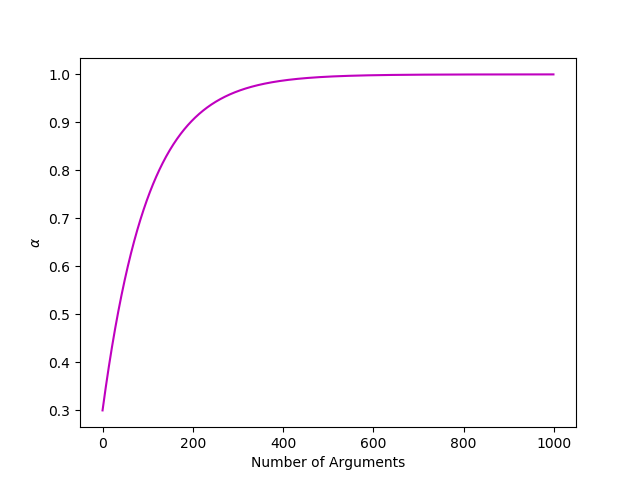
\includegraphics[width=0.49\textwidth]{Images/Misc/Stubbornness.png}
    \caption{A graph to show the rate at which agents change the importance they place on new information in the Stubborn Model. \textit{Using $\alpha_0 = 0.3, \lambda = 0.01$}}
    \label{fig:stubbornness_curve}
\end{figure}
\chapter{Analysis}\label{sect:analysis}

\section{Fixed Points Analysis} \label{sect:fixed_point_analysis}

All of the models in the previous chapter represent discrete time mappings. As such, it is therefore possible to identify fixed points so as to better understand the behaviour of some of the models. As in~\cite{Hegselmann2002OpinionSimulation}, it is challenging to provide analytical insights for some combinations of these models. However, the Open model can be readily analysed with Passive listeners.


For a fixed point in this system, it must hold that $\underline{\underline{\mathbf{P}}}^{t+1} = \underline{\underline{\mathbf{P}}}^t$. This equation requires that no agent has updated its beliefs and so the system is unchanged. The structure of the method defined at the beginning of~\cref{sect:method} dictates that, at most, one listener agent will update at any one iteration. Hence, at most only one row of matrix $\underline{\underline{\mathbf{P}}}^t$ will change and so can be considered in isolation. 

Without loss of generality, let us select two agents from $\underline{\underline{\mathbf{P}}}^t$ and label them $\underline{\mathbf{P}}_s$ and $\underline{\mathbf{P}}_l$ respectively. Hence, for all agents, a fixed point must satisfy

\begin{equation}
    \underline{\mathbf{P}}_l = \alpha \cdot \underline{\mathbf{P}}_l + (1 - \alpha) \cdot \underline{\mathbf{P}}_s. \label{eq:open_FP}
\end{equation}

There are two possible ways this can occur. Firstly, when $\alpha = 1$, we have a trivial fixed point. Secondly, assuming $\alpha < 1$, the fixed point occurs when $\underline{\mathbf{P}}_l=\underline{\mathbf{P}}_s$ for all possible pairs of agents. This reveals that it is likely that a fixed point will be found when the agents have converged to a single shared belief, a claim that is supported in simulation. To test the stability of these fixed points, we take the eigenvalues of the Jacobian of \cref{eq:open_FP} which gives $\alpha \underline{\underline{\mathbf{I}}}$. The system is stable when the modulus of all of the eivenvalues lie within the unit circle. The trivial fixed point is clearly stable as $\abs{\alpha} = 1$. The non-trivial fixed point $\underline{\mathbf{P}}_l=\underline{\mathbf{P}}_s$ is asymptotically stable as $\abs{\alpha} < 1$. This shows that, under this particular scheme, the agents are guaranteed to cluster together, converging upon a consensus. However, the existence of a stable fixed point does not guarantee that the population converges to a belief with absolute certainty. 

Perhaps more interesting is the case of Bottom Up speakers and Passive listeners. Using the same notation as above, the equation to reveal fixed points becomes

\begin{equation}
    \underline{\mathbf{P}}_l = \alpha \cdot \underline{\mathbf{P}}_l + (1 - \alpha) \cdot \frac{\underline{\mathbf{A}} \odot \underline{\mathbf{P}}_l}{\underline{\mathbf{A}} \cdot \underline{\mathbf{P}}_l}. \label{eq:BU_FP}
\end{equation}

From this equation, it can be shown that there are three fixed points. The first is trivial at $\alpha = 1$. The second occurs when $P_L(\mathbf{A}) = 0$ meaning that the listener has a $0$ probability for every state that the speaker has asserted and so does not update. The third occurs when $P_L(\mathbf{A}) = 1$, meaning that the speaker has asserted at least every state for which the listener has a non-zero probability. This final fixed point indicates that

\begin{align*}
    \underline{\mathbf{P}}_l = \frac{\underline{\mathbf{A}} \odot \underline{\mathbf{P}}_l}{\underline{\mathbf{A}} \cdot \underline{\mathbf{P}}_l}.
\end{align*}

This condition highlights two things: firstly, that $ \underline{\mathbf{A}} \cdot \underline{\mathbf{P}}_l = 1 $; secondly, that $ \underline{\mathbf{A}} \odot \underline{\mathbf{P}}_l =  \underline{\mathbf{P}}_l$. These are equivalent to $\sum^n_j A_j p_{l,j} = 1$ and $ p_{l,j} = A_j p_{l,j} $ respectively. 

As previously, to show the stability of these fixed points, the Jacobian must be computed. First, consider the diagonal elements of $\underline{\underline{\mathbf{J}}}$, given by

\begin{align}
    J_{a,a} = \frac{d f(p_{l,a})}{d p_{l,a}} &= \frac{d}{d p_{l,a}} \left( \alpha p_{l,a} + (1 - \alpha) \cdot \frac{A_a p_{l,a}}{\sum^n_j A_j p_{l,j}} \right) \\
    &= \alpha + (1 - \alpha) \cdot \left( \frac{A_a}{\sum^n_j A_j p_{l,j}} - \frac{A_a^2 p_{l,a}}{\sum^n_j A_j p_{l,j}} \right) \\
    &= \alpha + (1 - \alpha) \cdot \frac{A_a}{\sum^n_j A_j p_{l,j}} \left( 1 - \frac{A_a p_{l,a}}{\sum^n_j A_j p_{l,j}} \right), \\ 
\end{align}

and off-diagonals are given by

\begin{align}
    J_{a,b} = \frac{d f(p_{l,a})}{d p_{l,b}} &= \frac{d}{d p_{l,b}} \left( \alpha p_{l,a} + (1 - \alpha) \cdot \frac{A_a p_{l,a}}{\sum^n_j A_j p_{l,j}} \right) \\
    &= 0 + (1 - \alpha) \cdot \left( - \frac{A_a p_{l,a} A_b}{\sum^n_j A_j p_{l,j}} \right). \\
\end{align}


When $\alpha = 1$, it can be seen that off-diagonals are $0$, and the diagonal elements are $1$, therefore the eigenvalues of $\underline{\underline{\mathbf{J}}}$ are $1$. When $P_L(\mathbf{A}) = 0$, the diagonal elements of $\underline{\underline{\mathbf{J}}}$ are $\alpha$, however, the off-diagonals are not so clear. Consider the full $n \times n$ real matrix

\begin{center}
$\underline{\underline{\mathbf{J}}} = \begin{bmatrix}
    \alpha - (1 - \alpha) A_1 (1- p_{l,1}) & - (1 - \alpha) A_1 p_{l,2} & \dots  & -(1 - \alpha) A_1 p_{l,n} \\
    - (1 - \alpha) A_2 p_{l,1} &  \alpha - (1 - \alpha) A_2 (1- p_{l,2}) &  \dots  & -(1 - \alpha) A_2 p_{l,n} \\
    \vdots & \vdots & \ddots & \vdots \\
    - (1 - \alpha) A_n p_{l,1} & - (1 - \alpha ) A_n p_{l,2} &  \dots & \alpha - (1 - \alpha) A_n (1- p_{l,n}) \\

\end{bmatrix}$.
\end{center}

For stability, the modulus of the eigenvalues of this matrix must lie within the unit circle, however, it is not possible to evaluate each eigenvalue in the general case for $n>5$, due to the Abel-Ruffini Theorem~\cite{Abel1824MemoireDegre}. With some minor manipulations to this matrix, it is possible to apply Perrón-Frobenius theorem to calculate the largest positive real eigenvalue, but this is insufficient for determining the stability, as there is no guarantee that all the eigenvalues are real~\cite{Perron1907ZurMatrices}. Fortunately, Gershgorin Circle Theorem provides a method for bounding the location of the eigenvalues in the complex plane~\cite{Gerschgorin1931UberMatrix}. This theorem states that each eigenvalue $\lambda_a$ of an $n\times n$ square matrix $\underline{\underline{\mathbf{M}}}$ will lie within at least one Gershgorin Disc $D(m_{a,a}, R_a)$ where the centre of the disc $m_{a,a}$ is the $a^\textnormal{th}$ element on the diagonal of $\underline{\underline{\mathbf{M}}}$, and its radius $R_a = \sum^n_{b \neq a}\abs{m_{a,b}}$. Consider \cref{fig:gershgorin}. This figure shows the unit circle in the complex plane and three Gershgorin Discs. If all of the discs were within the unit circle, our system would be stable. It should be noted that, because the eigenvalues must lie within at least one of these discs, having a disc outside the unit circle is a necessary but not sufficient condition for determining that the system is unstable. \\


\begin{figure}
\begin{center}
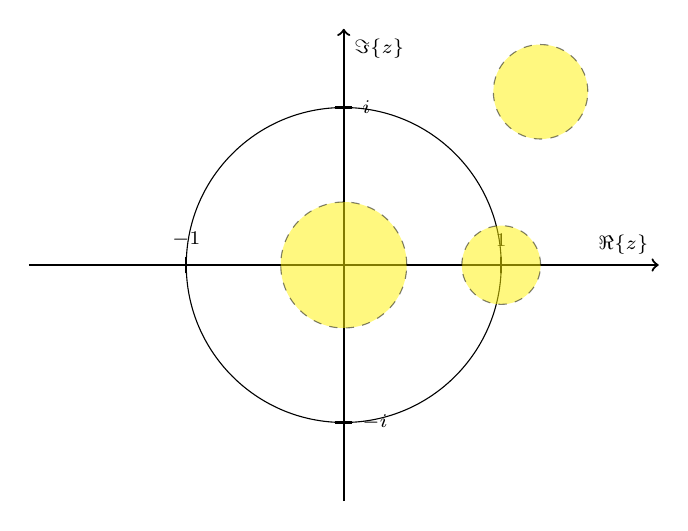
\begin{tikzpicture}
     \begin{scope}[thick,font=\scriptsize]
     % Axes:
     % Are simply drawn using line with the `->` option to make them arrows:
     % The main labels of the axes can be places using `node`s:
     \draw [->] (-4,0) -- (4,0) node [above left]  {$\Re\{z\}$};
     \draw [->] (0,-3) -- (0,3) node [below right] {$\Im\{z\}$};
 
     % Axes labels:
     % Are drawn using small lines and labeled with `node`s. The placement can be set using options
     \iftrue% Single
     % If you only want a single label per axis side:
     \draw (2,-3pt) -- (2,3pt)   node [above] {$1$};
     \draw (-2,-3pt) -- (-2,3pt) node [above] {$-1$};
     \draw (-3pt,2) -- (3pt,2)   node [right] {$i$};
     \draw (-3pt,-2) -- (3pt,-2) node [right] {$-i$};
     \else% Multiple
     % If you want labels at every unit step:
     \foreach \n in {-4,...,-1,1,2,...,4}{%
         \draw (\n,-3pt) -- (\n,3pt)   node [above] {$\n$};
         \draw (-3pt,\n) -- (3pt,\n)   node [right] {$\n i$};
     }
     \fi
     \end{scope}
     % The circle is drawn with `(x,y) circle (radius)`
     % You can draw the outer border and fill the inner area differently.
     % Here I use gray, semitransparent filling to not cover the axes below the circle
     \path [draw=black] (0,0) circle (2);
     \path [draw=black, dashed, fill=yellow, semitransparent] (0,-0) circle (0.8);
     \path [draw=black, dashed, fill=yellow, semitransparent] (2,0) circle (0.5);
     \path [draw=black, dashed, fill=yellow, semitransparent] (2.5,2.2) circle (0.6);
     % Place the equation into the circle:
\end{tikzpicture}
\end{center}
\caption{A plot of an Argand diagram demonstrating Gershgorin Circle Theorem. The system is stable if the eigenvalues are all within the unit circle, shown in black. The yellow circles show Gershgorin discs of a system. The theorem dictates that each eigenvalue must lie within at least one of these discs. }
\label{fig:gershgorin}
\end{figure}

Therefore, for the fixed point $P_L(\mathbf{A}) = 0$, the eigenvalues lie within Gershgorin Discs of the form 

\begin{align}
    &D(\alpha, \sum_{b \neq a}^n \abs{ - (1 - \alpha) A_a p_{l,b} } ) \nonumber \\
    &D(\alpha, \sum_{b \neq a}^n (1 - \alpha) A_a p_{l,b} ) \nonumber \\
    &D(\alpha, (1 - \alpha) A_a (1 - p_{l,a}) ) .
\end{align}

Here, as $\underline{\mathbf{A}}$ is a binary vector, this equation can be broken down into two cases. Firstly, let $A_a = 0$. In this case, the disc becomes $D(\alpha, 0)$, which is within the unit circle. Secondly, let $A_a = 1$. In this case, $p_{l,a} = 0$, and therefore the disc becomes $D(\alpha, 1-\alpha)$, which makes contact with, but does not cross, the unit circle. Hence, for $P_L(\mathbf{A}) = 0$, the fixed point is stable. 

A similar argument exists for the fixed point at $P_L(\mathbf{A}) = 1$. Here, the eigenvalues of $\underline{\underline{\mathbf{J}}}$ must lie within discs of the form 

\begin{align}
 D(\alpha - ( 1 - \alpha ) A_a ( 1 - p_{l,a}), \sum_{b \neq a}^n \abs{ - (1 - \alpha) A_a p_{l,b} }) \nonumber\\
 D( \alpha - (1 - \alpha) A_a (1 - p_a), (1 - \alpha) A_a (1 - p_{l,a})).  
\end{align} \label{eq:2FPGershgorin}

As $\underline{\mathbf{A}}$ is a binary vector, we can split~\cref{eq:2FPGershgorin} into two different types of disc, one in which $A_a = 0$ and one in which $A_a = 1$. When $A_a = 0$, the discs are $D(\alpha, 0)$, and so are within the unit circle. When $A_a = 1$, the discs are given by \[ D(\alpha + (1 - \alpha) (1 - p_{l,a}), (1 - \alpha)(1 - p_{l,a})).\] Therefore, the system is stable when \[ \alpha + 2(1 - \alpha)(1 - p_{l,a}) \leq 1.   \]

This simplifies to 
\begin{align}
    \alpha + 2(1 - \alpha) ( 1- p_{l,a}) & \leq 1 \nonumber  \\
    2(1 - \alpha - p_{l,i} + \alpha p_{l,i}) & \leq 1 - \alpha \nonumber\\
    - 2p_{l,a} + 2\alpha p_{l,a} & \leq \alpha - 1 \nonumber \\
    2 p_{l,a} (\alpha - 1) & \leq \alpha - 1 \nonumber \\
    p_{l,a}  & \geq \frac{1}{2}.
\end{align}

Hence, when $A_a = 0$, each corresponding disc is within the unit circle and when $A_a = 1$, the system as a whole is guaranteed to be stable when $p_{l,a} \geq \frac{1}{2}$. This can only happen in one of two ways: $p_{l,a} = 1$ and all other probabilities are $0$, or there are two states for which $p_{l,a} = \frac{1}{2}$. Therefore, it is expected that the system will tend to steady states in which, for every agent, either $p_{l,a} = 1 \textnormal{ or } p_{l,a} = \frac{1}{2}$. Therefore, it is expected that the agents will graduate toward either certainty in a single state of the world or equal levels of uncertainty in two states. 





\section{Simulation Experiments}

The following experiments were run on an Intel(R) Core i7-8650 CPU 1.90Ghz with the following parameters as default, unless otherwise stated: $n=3, K=100, \alpha = 0.3, \gamma = 0.5, t_{max} = 50,000, \eta = 10^{-5}, T=3$. Error bars are shown at $\pm \sigma$, one standard deviation. 
\subsection{Consensus}

To gain an insight into the dynamics of these systems, let us consider their entropy, as defined in~\cref{eq:shannon_entropy}. This serves as a measure of the uncertainty in the system. High values imply the absence of strong beliefs in the population, and low values imply a level of certainty, though importantly, not consensus. To illustrate the distinction between these entropy values, consider \cref{fig:2d-simplex}. There are some agents in the corners of the Barycenter plot that are initialised with strong beliefs in one states of the world. These agents will have low entropy values, whereas those closer to the centre of the plot will have much higher entropy values due to their uncertainty. 


\Cref{fig:entropy_all,fig:J-div_all} show plots of entropy and J-Divergence changing over time for each of the four models proposed. Here, the listeners are Passive. In can be seen that the entropy and the J-Divergence of the Open model follow significantly different trajectories to the other models. The J-Divergence decreases, as in the other models, although it reaches $0$ almost immediately. This suggests that the agents cluster together rapidly. The entropy plot, however, differs significantly to the other models. It can be seen to increase to a value of $\approx 1.09$. This is approximately the maximum entropy value that could be obtained in a $3$-dimensional world. It is apparent that the agents quickly cluster together, each of them assuming the uniform distribution as their beliefs. This is due to their uniformly random initialisation, not a characteristic of the model. Therefore, the Open model behaves as predicted by~\cref{sect:fixed_point_analysis}, converging to a single point that is approximately the average of every agent's beliefs. It should be noted that there is limited variation in the behaviour of the Open model, as evidenced by the narrow error bars. 

\begin{figure}[H]
 \centering
  \begin{minipage}[ht]{0.49\textwidth}
    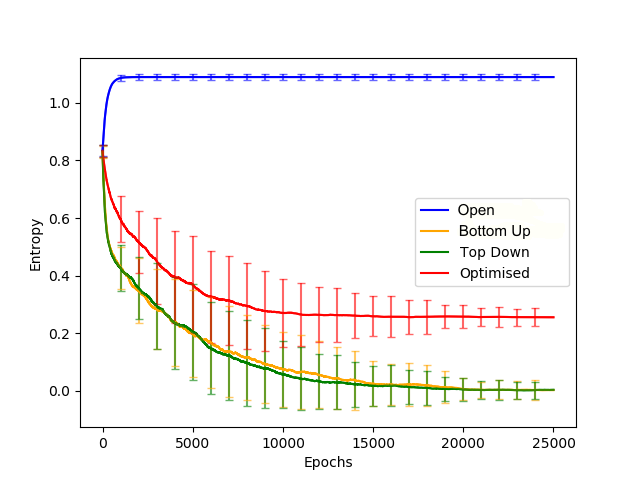
\includegraphics[width=\textwidth]{Images/Figures/All/Entropy_25000.png}
    \subcaption{Entropy}\label{fig:entropy_all}
 \end{minipage}
 \hfill
 \begin{minipage}[ht]{0.49\textwidth}
    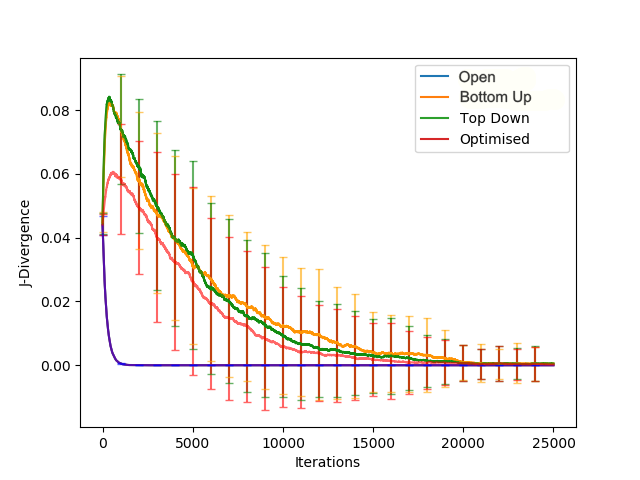
\includegraphics[width=\textwidth]{Images/Figures/All/J-Div_25000.png}
    \subcaption{J-Divergence}\label{fig:J-div_all}
 \end{minipage}
 \caption{Two plots to show the change in entropy and J-Divergence over time, for the Open, Bottom Up, Top Down, and Optimised models. These plots were obtained using Passive listeners, and were averaged over $100$ runs.}
\end{figure}

The Bottom Up and Top Down models seem to behave indistinguishably, both reducing the uncertainty in the population as time passes, tending toward $0$ at a similar rate for both entropy and J-Divergence. These two approaches are capable of achieving a population of agents that are certain of one state alone. In order to determine whether one is a dominant strategy, the two models must be compared across a variety of different parameter values, explored in the following section.  It should be noted that all models other than the Open model appear to \emph{increase} the disagreement between agents for the first few hundred iterations. This occurs at the same time as the gradient of the entropy plot is maximal. At this time, agents are quickly persuaded toward one particular state, depending on the arguments they hear. Due to the random initialisation, this divides the population, increasing the J-Divergence until a majority forms in support of one possible state and the agents begin to converge toward it. In simulation, this phenomenon manifests in some interesting patterns such as those shown in~\cref{fig:sierpinski_triangle_intro}. 


\begin{figure}[H]
    \centering
    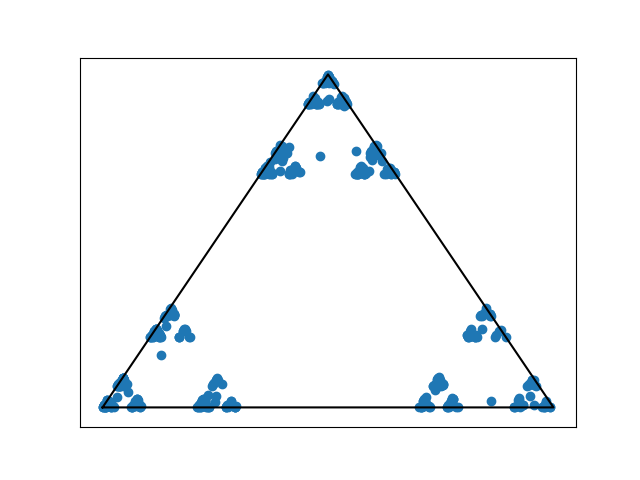
\includegraphics[width=0.45\textwidth]{Images/Figures/Barycenter/Serpinski_example.png}
    \caption{The $500^\textnormal{th}$ iteration of a simulation of the Bottom Up model. $500$ agents are shown, with clusters of agents forming at $\underline{\mathbf{P}}^t_{x} \approx [\alpha, 1-\alpha, 0]^T$. The listeners are Passive. Importantly, the system has not converged at this point.}
    \label{fig:sierpinski_triangle_intro}
\end{figure}

When a listener that has a strong belief in $H_j$ is presented with an assertion $ \mathbf{A} = \{ H_{¬j} \}$, approximately the following update occurs. 


\begin{center}
$\underline{\mathbf{P}}^t_l = \alpha \begin{bmatrix}
    1-\epsilon\\
    \epsilon\\
    0
\end{bmatrix} + (1 - \alpha) \frac{\begin{bmatrix} 0\\1\\0 \end{bmatrix} \odot \begin{bmatrix} 1-\epsilon\\ \epsilon\\ 0 \end{bmatrix}} {\begin{bmatrix} 0\\1\\0 \end{bmatrix} \cdot \begin{bmatrix} 1- \epsilon\\ \epsilon \\ 0\end{bmatrix}} $, \\
\end{center}
where $\epsilon$ is an arbitrarily small positive number, such that $\sum^n_j p^t_{l,j} = 1$. Then 
\begin{center}
$\underline{\mathbf{P}}^t_l =\alpha \begin{bmatrix}
    1 - \epsilon \\
    \epsilon\\
    0
\end{bmatrix} + (1 - \alpha) \begin{bmatrix} 0\\ 1 \\ 0  \end{bmatrix} $ \\

$\underline{\mathbf{P}}^t_l \approx \begin{bmatrix} \alpha \\ 1 - \alpha \\ 0  \end{bmatrix}$.
\end{center}

As an aside, when $\alpha = 0.5$, the plot shows remarkable similarity to the Sierpinski Triangle due to the same phenomenon as~\cref{fig:sierpinski_triangle_intro}, demonstrated in~\cref{fig:sierpinski_compare}. 

\begin{figure}[H]
  \begin{minipage}[t]{0.49\textwidth}
    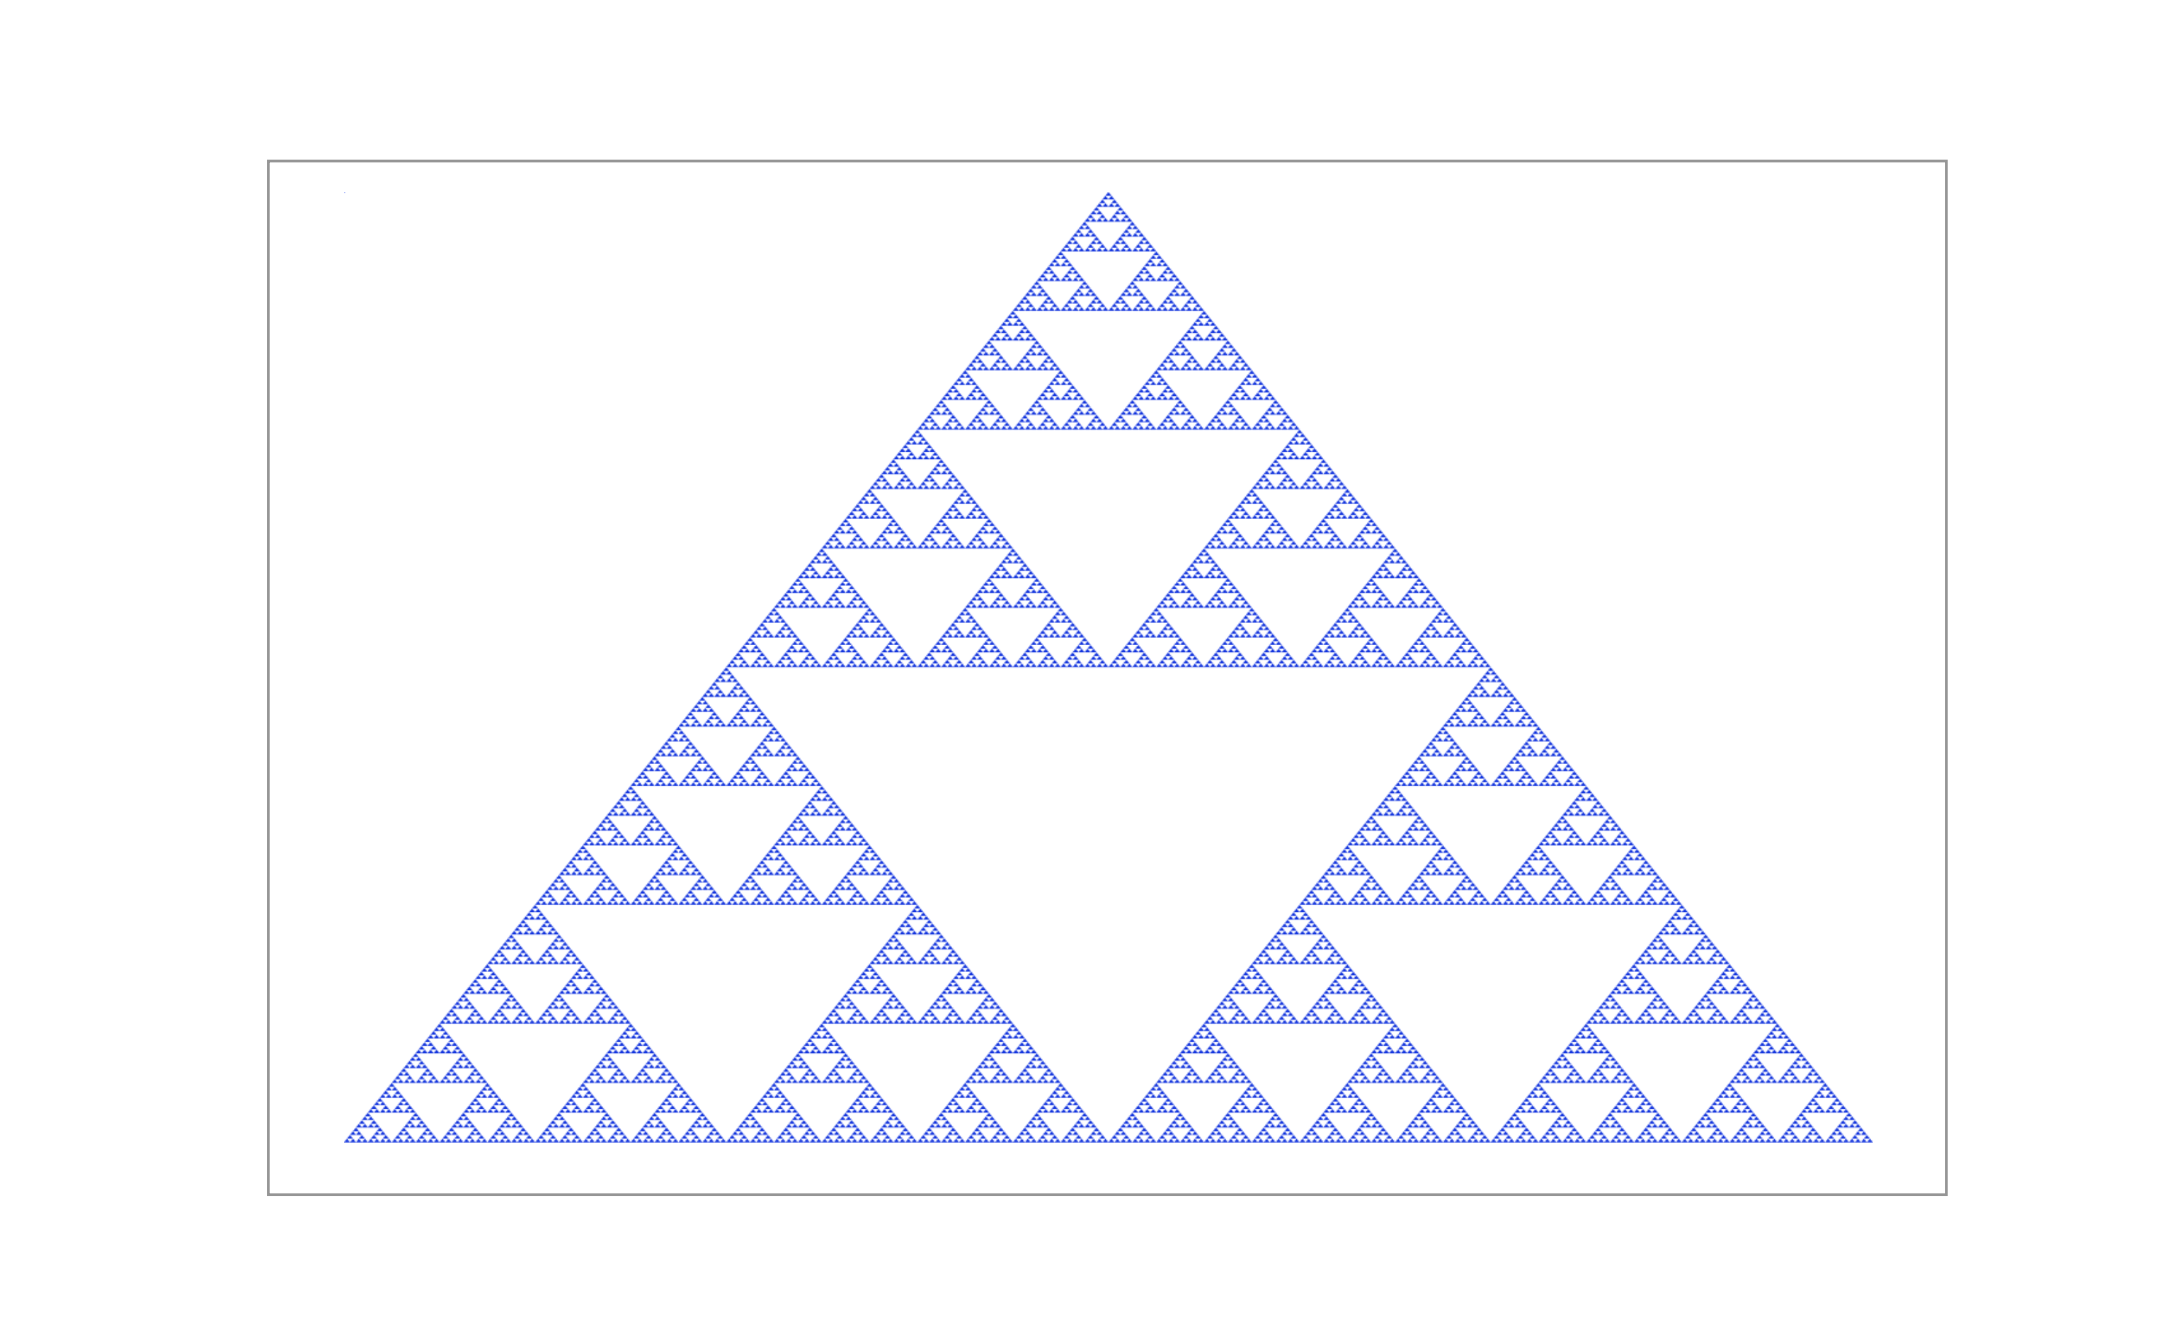
\includegraphics[width=\textwidth]{Images/Misc/Sierpinski_triangle_real_resized.png}
    \subcaption{Sierpinski Triangle}
  \end{minipage}
  \hfill
 \begin{minipage}[t]{0.49\textwidth}
    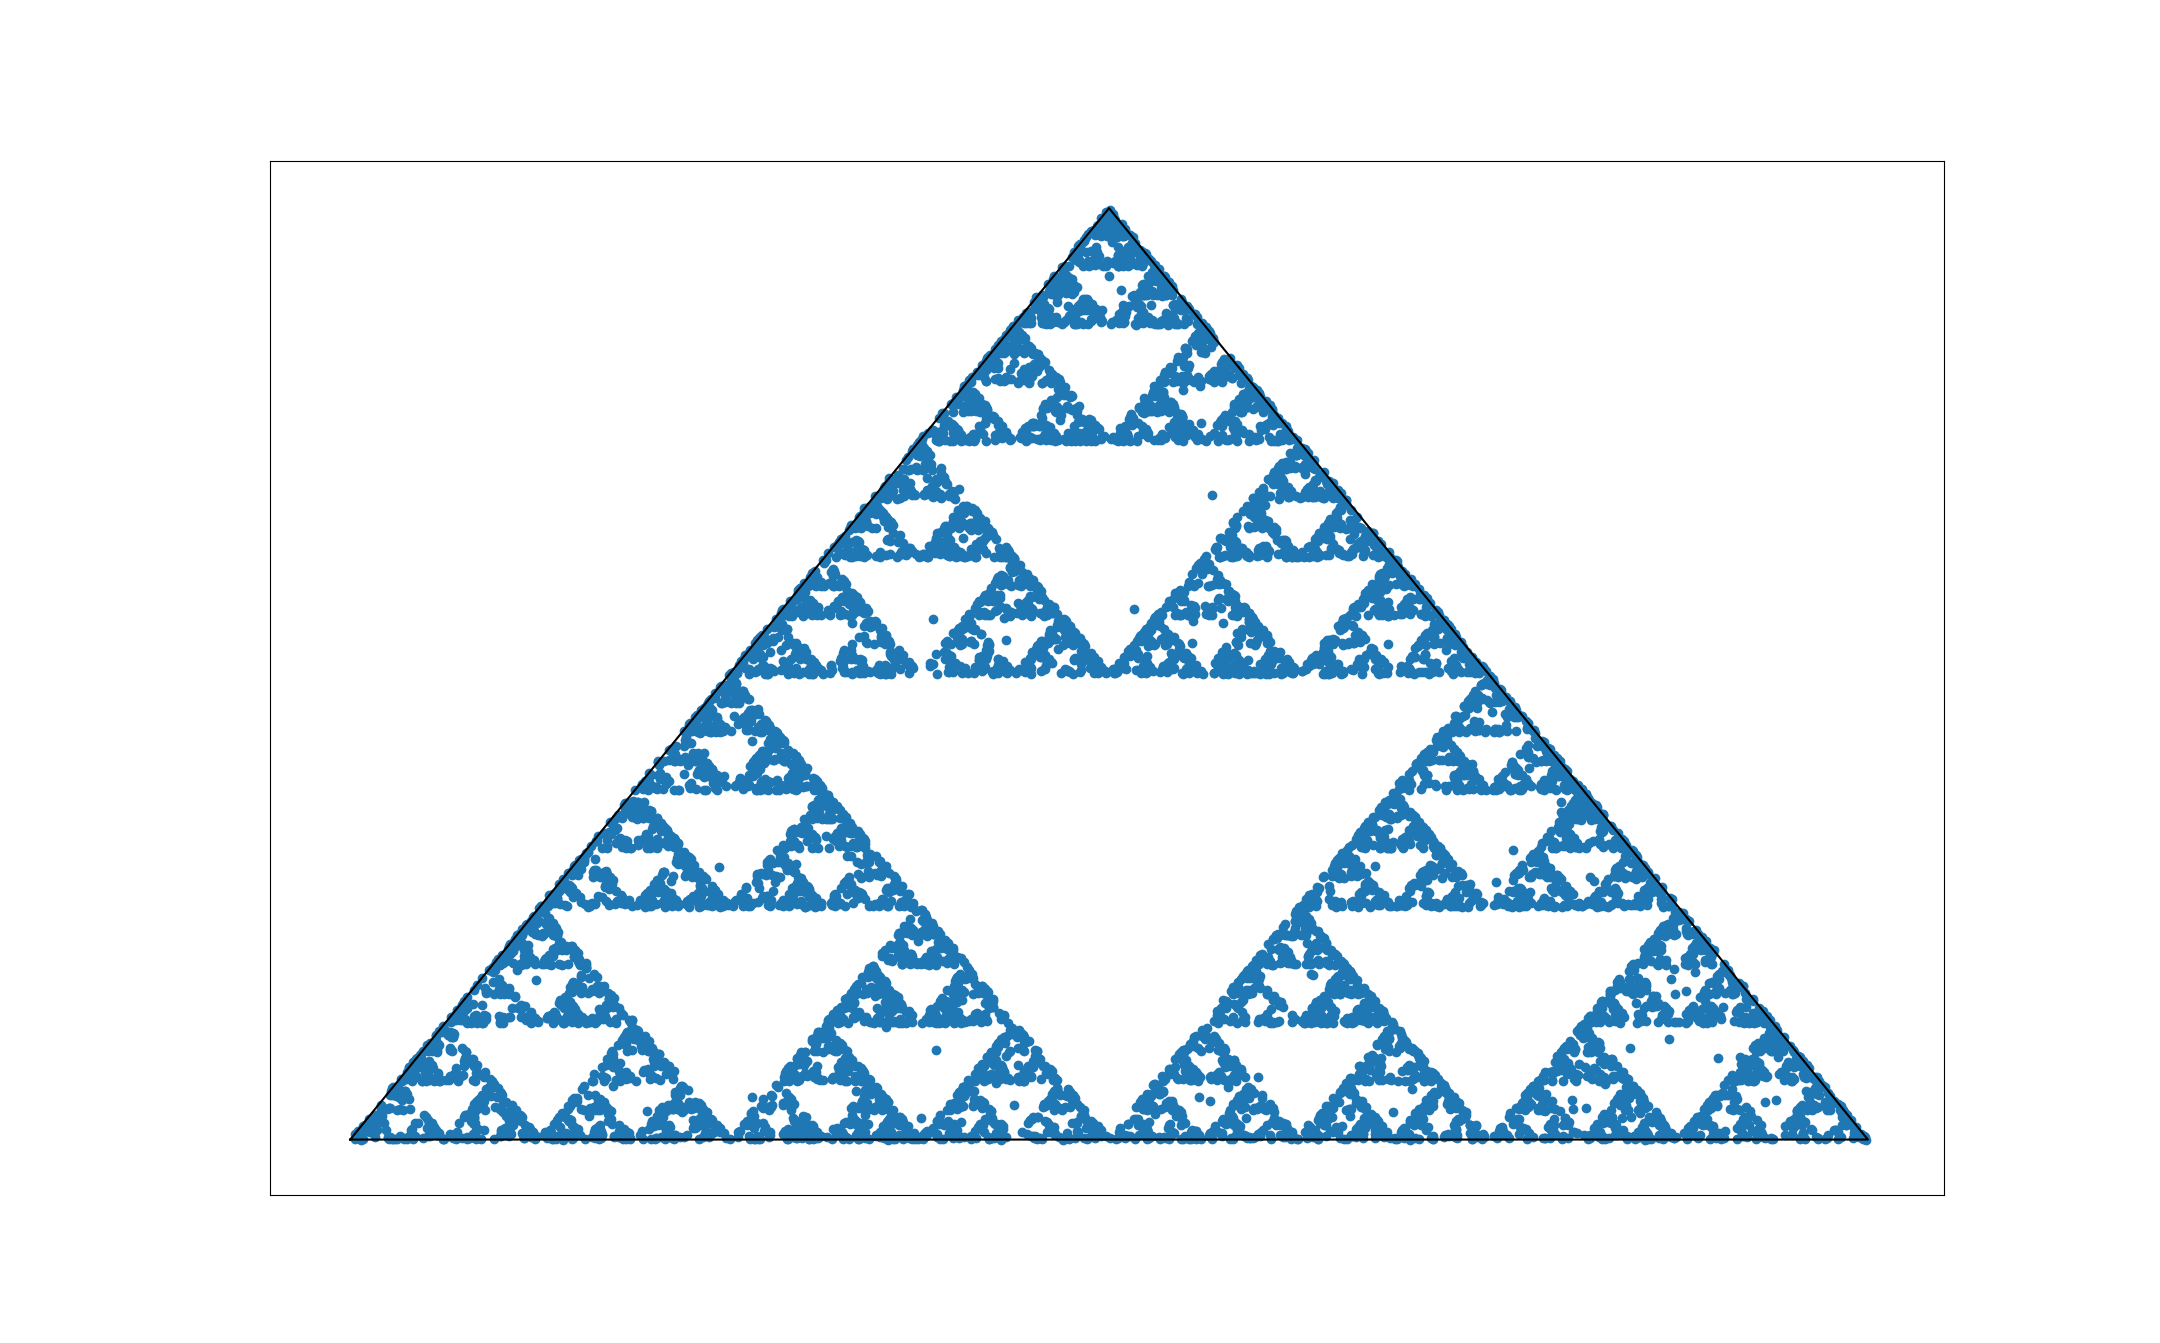
\includegraphics[width=\textwidth]{Images/Figures/Barycenter/Serpinski_BU.png}
    \subcaption{Bottom Up Model} \label{fig:sierpinski_BU}
 \end{minipage}
 \caption{ The true Sierpinski Triangle, and the Bottom Up model after $80,000$ iterations with $K=10,000, \alpha=0.5$. The pattern in (b) is not stable and breaks down with time. \\ \textit{Image downloaded from \url{https://bit.ly/2GkoUXI}}  }\label{fig:sierpinski_compare}
\end{figure}


The population in the Bottom Up model forms a particular structure, as shown in~\cref{fig:sierpinski_BU}. The explanation for this structure arises due to the similarity between the update rule and a chaos game. Originally described by Barnsley, a chaos game
\begin{displayquote} 
    ``\dots is a Markov Chain Monte Carlo algorithm that is applied in order to describe probability distributions supported on an attractor of an iterated function system''~\cite{Barnsley2011ChaosSpaces}.
\end{displayquote}

To better understand them, an example of a chaos game is taken from \cite{Feldman.DavidP2012ChaosIntroduction} that bears a resemblance to the general speaker-listener model described in~\cref{sect:method}. In his book, Feldman begins by selecting a point anywhere within the outermost triangle shown in \cref{fig:chaos_game}. Then, if such a device were practical, a three-sided die is rolled, and the point is moved half-way toward the result of the roll. For example, let the first die roll be a $2$. The point would then move to be within the upper shaded triangle, labelled ``$2$''. If the subsequent roll was a $3$, then the point would lie anywhere within the triangle, marked ``$2,3$''. This process can be repeated ad infinitum creating infinitely dense trajectories of this point, as well as revealing areas that it is impossible for the point to reach, shown in white. After an infinite number of iterations, the trajectory of this point will reveal the Sierpinski triangle. Similar results are obtained using the update rule for Passive listeners in which agents update their beliefs toward a vertex that, at least in the early stages of the population's communications, is chosen almost uniformly at random. However, as soon as a large cluster of agents forms, the balance of probability shifts toward them, so the fractal structure of the population begins to break down. In the Optimised model, occasionally the largest cluster can form at a vertex of one of the sub-triangles and remain there, as shown in~\cref{fig:optimised_problem_case}. A further difference is that Passive listeners update toward the vertex by some function $f(\alpha)$, instead of the point moving half-way toward the selected vertex.  

\begin{figure}[]
\begin{center}
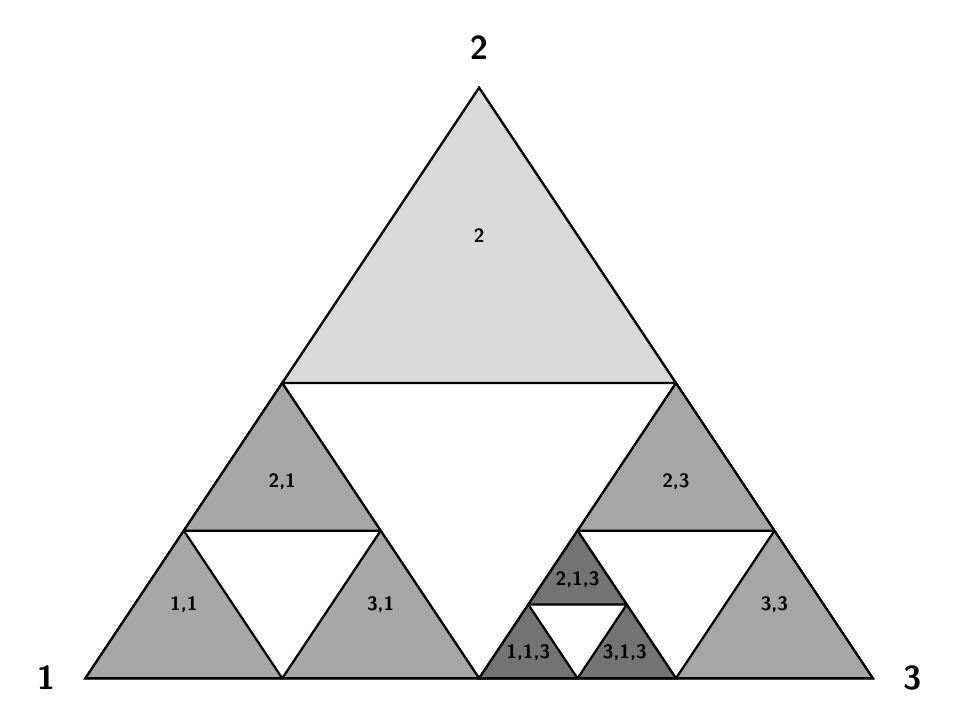
\begin{tikzpicture}
    \draw[thick] (0,0) -- (10,0) -- (5,7.5) -- cycle;
    
    \draw[thick] (0,0) -- (5,0) -- (2.5,3.75) -- cycle;  
    \draw[thick] (10,0) -- (5,0) -- (7.5,3.75) -- cycle;
    \draw[thick, fill=black!15] (2.5,3.75) -- (7.5,3.75) -- (5,7.5) -- cycle;

    
    \draw[thick, fill=black!35] (0,0) -- (2.5,0) -- (1.25,1.875) -- cycle;
    \draw[thick, fill=black!35] (2.5,0) -- (5,0) -- (3.75,1.875) -- cycle;
    \draw[thick, fill=black!35] (1.25,1.875) -- (3.75,1.875) -- (2.5,3.75) -- cycle;
    \draw[thick] (5,0) -- (7.5,0) -- (6.25,1.875) -- cycle;
    \draw[thick, fill=black!35] (7.5,0) -- (10,0) -- (8.75,1.875) -- cycle;
    \draw[thick, fill=black!35] (6.25,1.875) -- (8.75,1.875) -- (7.5,3.75) -- cycle;
    
    
    \draw[thick, fill=black!55] (5,0) -- (6.25,0) -- (5.625,0.9375) -- cycle;
    \draw[thick, fill=black!55] (6.25,0) -- (7.5,0) -- (6.875,0.9375) -- cycle;
    \draw[thick, fill=black!55] (5.625,0.9375) -- (6.875,0.9375) -- (6.25,1.875) -- cycle;

    \node at (5,5.625) {\scriptsize\textbf{2}};
    \node at (5,8) {\large\textbf{2}};
    \node at (-0.5,0) {\large\textbf{1}};
    \node at (10.5,0) {\large\textbf{3}};
    
    \node at (1.25,0.9375) {\scriptsize\textbf{1,1}};
    \node at (2.5, 2.5) {\scriptsize\textbf{2,1}};
    \node at (3.75, 0.9325) {\scriptsize\textbf{3,1}};
    
    \node at (7.5, 2.5) {\scriptsize\textbf{2,3}};
    \node at (8.75, 0.9325) {\scriptsize\textbf{3,3}};
    
    \node at (5.625, 0.32625) {\scriptsize\textbf{1,1,3}};
    \node at (6.25, 1.25) {\scriptsize\textbf{2,1,3}};
    \node at (6.85, 0.32625) {\scriptsize\textbf{3,1,3}};

\end{tikzpicture}
\end{center}
\caption{A pictorial representation of a chaos game to generate a Sierpinski Triangle. A point is chosen at random from the outermost triangle then, at each iteration, is updated half-way toward a randomly selected vertex. The triangle marked ``$3,1,3$'' represents the area that the randomly selected first point must be in if the sequence of vertices has been first $3$, then $1$ then $3$. Repeated ad infinitum, this process will generate a Sierpinski Triangle.}  \label{fig:chaos_game}
\end{figure}

Finally, the Optimised model appears to be failing to live up to its name. While it does induce a reduction in the entropy of the system, it does not enable the agents to become certain that any one state is true. That said, the agents do arrive at a consensus, as evidenced by the J-Divergence plot. This indicates that the agents converge to a single point in probability space, but that that point is not in a corner of the Barycenter plot, and thus the agents are not certain in a single state. \Cref{fig:optimised_problem_case} shows a histogram of the final states of agents using the Optimised approach. 

\begin{figure}[]
    \centering
    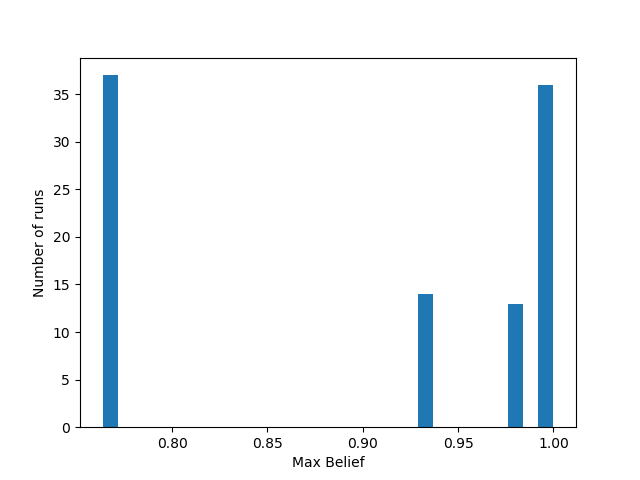
\includegraphics[width=0.59\textwidth]{Images/Figures/Optimised/ChaoticAttractorMaybe.png}
    \caption{ A histogram showing the maximum probability at the $25,000^\textnormal{th}$ iteration of the Optimised model, for $100$ runs. It can be seen that there are two main locations the agents converge to, with other, less frequent possibilities in between.  }
    \label{fig:optimised_problem_case}
\end{figure}

\Cref{fig:optimised_problem_case} shows a histogram of $100$ runs at $\alpha =0.3$, with the maximum probability of the agents at steady state on the $x$-axis. It can be seen that the maximum probability values are not random, instead, clustering together at particular values, approximately $0.76, 0.93, 0.98$ and $1$. The differences between these values consecutively can be approximated to $\frac{1}{3}$ multiplied by the difference between the previous pair of probabilities. This ratio is $\approx \alpha$, suggesting that the Optimised model does not always converge to a vertex of the Barycenter plot, instead converging to a vertex of one of the sub-triangles shown in~\cref{fig:chaos_game}. 

In order to better understand why this happens, we must return to the objective function of this model. Since the speaker seeks to minimise the J-Divergence between itself and the listener, at this final state, the speaker has two options. If it were to assert the single most probable state, the listener would likely become more certain in that single state, gradually allowing the population to become certain in a single state of the world. However, if the speaker were to assert that singleton, the J-Divergence between the speaker and listener would clearly increase, so it is optimal for the speaker to assert something that does not cause the listener to move away, even if this were to improve the collective certainty. From this analysis, it is clear that the Optimised model is, in fact, sub-optimal, showing that unconstrained speakers are detrimental to the decision-making abilities of the group. 



\subsection{Convergence}

In order to compare the behaviour of the Bottom Up and Top Down models, let us examine their convergence across the variation of $\gamma$ between $0$ and $1$. The Open and Optimised models are unaffected by $\gamma$ and so have not been included. Recall that the system is said to have converged if $\Delta \hat{E}^{T+t} = \abs{ \hat{E}^t -  \hat{E}^{t+T}}  \leq \eta$. \Cref{fig:convergence_none} shows the results. 

\begin{figure}[h!]
 \centering
  \begin{subfigure}[ht]{0.45\textwidth}
    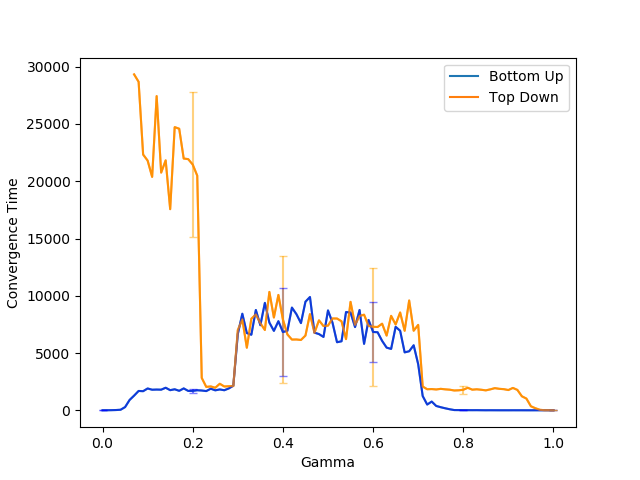
\includegraphics[width=\textwidth]{Images/Figures/BU+TD/None/Convergence_best.png}
    \caption{Convergence}\label{fig:convergence}
 \end{subfigure}
 \hfill
 \begin{subfigure}[ht]{0.45\textwidth}
    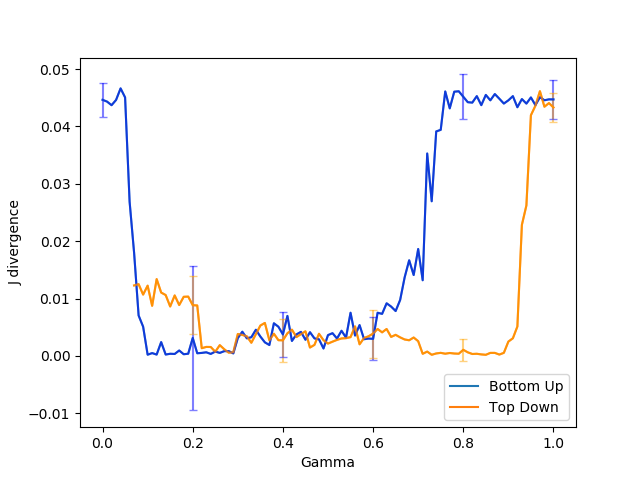
\includegraphics[width=\textwidth]{Images/Figures/BU+TD/None/J-Div_best.png}
    \caption{J-Divergence}\label{fig:J-Div_convergence}
 \end{subfigure}
 \hfill
 \begin{subfigure}[ht]{0.45\textwidth}
    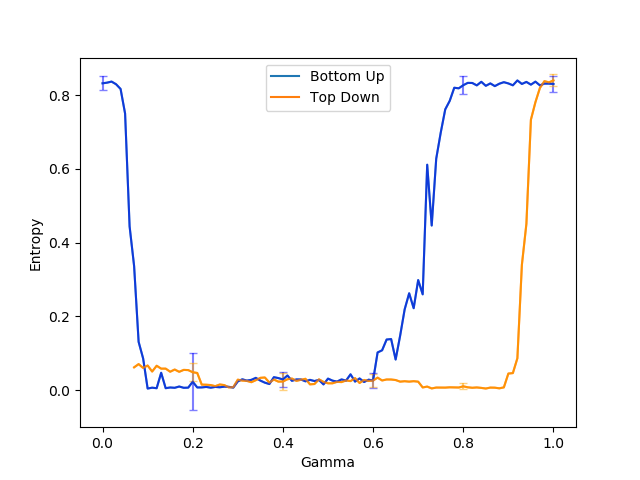
\includegraphics[width=\textwidth]{Images/Figures/BU+TD/None/Entropy_best.png}
    \caption{Entropy}\label{fig:entropy_convergence}
 \end{subfigure}
 \caption{ Three plots showing the convergent behaviour of the Bottom Up and Top Down models with Passive listeners as $\gamma$ is varied. (a) shows the time to convergence as defined by~\cref{eq:convergence}. (b) shows the average J-Divergence of the system at the corresponding iteration of (a). (c) shows the average entropy of the system at the corresponding iteration of (a). If the system has not converged within $50,000$ iterations, the point is left blank. }\label{fig:convergence_none}
\end{figure}

It is apparent that, for both models, high values of $\gamma$ relate to very rapid convergence. This can be attributed to the fact that at values of $\gamma \approx 1$, it is impossible for either model to create a meaningful assertion; they are limited to asserting $\emptyset$ in the Bottom Up model and $\mathbf{W}$ in the Top Down. Neither of these assertions produces any change in the listener. This registers as rapid convergence as the entropy remains constant coinciding with the increases in entropy and J-Divergence for $\gamma > 0.8$.

In the Bottom Up plots, one can observe rapid convergence for values of $\gamma \geq 0.6$. At this point, it is impossible for the speaker to assert anything other than a singleton, meaning that its arguments are guaranteed to be precise. This phenomenon increases the rate of convergence. Furthermore, as $\gamma$ increases, the only agents that can put forward any non-trivial argument are those who already hold extreme beliefs with high probability in one particular state. This accelerates the movement of the general population toward the region in which only extremist speakers can speak until more and more of the population holds similarly strong beliefs. This effect accelerates as more agents become able to assert something. 

It is also possible to observe a sharp increase in convergence time shortly after $ \gamma = \frac{1}{n}$. As $\gamma$ increases above this point, it begins to create a region of probability space in which it is impossible for an agent to assert anything, making them purely passive. For instance, if $\mathbf{P}_S =\{ 0.3, 0.3, 0.4\}$ and $\gamma = 0.5$, it is impossible for the speaker to assert anything. This will increase the convergence time as, if such an agent is picked, it is incapable of asserting anything meaningful. Meanwhile, the agents that can speak are likely to be asserting slightly general statements so convergence is slow until $\gamma$ approaches $0.6$. In the region $0.3 \leq \gamma \leq 0.6$, it can be seen that both models behave similarly, both converging within $7,500$ iterations. 

The Top Down approach exhibits some different behaviour with slow convergence times for low values of $\gamma$. The slow convergence for low $\gamma$ is attributable to oscillations in the dynamics of the system. At these values, it becomes possible for the agents to assert states for which they have very little probability. This delays convergence by convincing listening agents to update their probability distributions in a way that increases the distance between the speaker and listener. 

The intermediate values of $\gamma$ show slightly slower convergence times for both models. They both appear to converge to a population of agents that agree in a single state, as the entropy and J-Divergence are both close to $0$. Furthermore, it can be seen that the Bottom Up approach is the most affected by high values of $\gamma$, as such values place a harsh constraint on the assertions of the speaker. The Top Down model is shown to be more robust to changes in $\gamma$, with the majority of the agents holding strong beliefs in the same single possible world at steady state.  


\subsection{Analysis of Listener Models}

The previous analyses only utilise Passive listeners. In the following, we explore the effects of introducing the other types of listener we defined in~\cref{sect:method}. In order to maintain parity between the speaker and listener behaviour, the Discerning and Backfiring models disagree with an assertion if it fails to satisfy the reversal of the process that created it. To analyse these models, the above figures have been replicated with different listener models. \Cref{fig:convergence_FIE} shows the convergence of discerning listeners. It should be noted that, as soon as $\gamma > 0$ for the Bottom Up model and $\gamma < 1$ for the Top Down, a listener that is certain in a state $H_j$ is unable to update on an assertion $\{ H_{¬j} \}$


\begin{figure}[h!]
 \centering
  \begin{subfigure}[ht]{0.45\textwidth}
    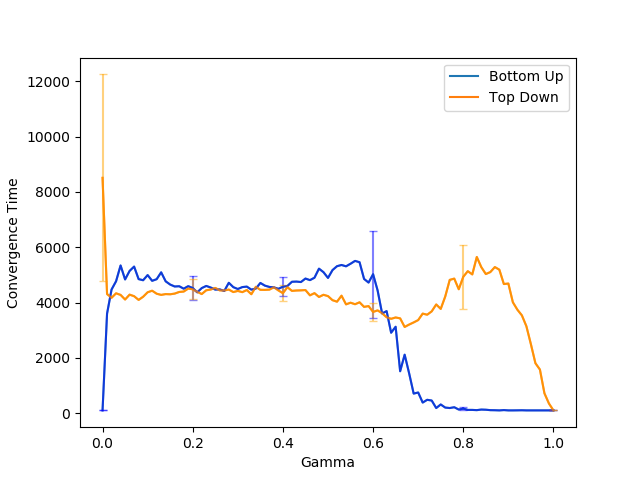
\includegraphics[width=\textwidth]{Images/Figures/BU+TD/FIE/Convergence_better.png}
    \caption{Convergence}
 \end{subfigure}
 \hfill
 \begin{subfigure}[ht]{0.45\textwidth}
    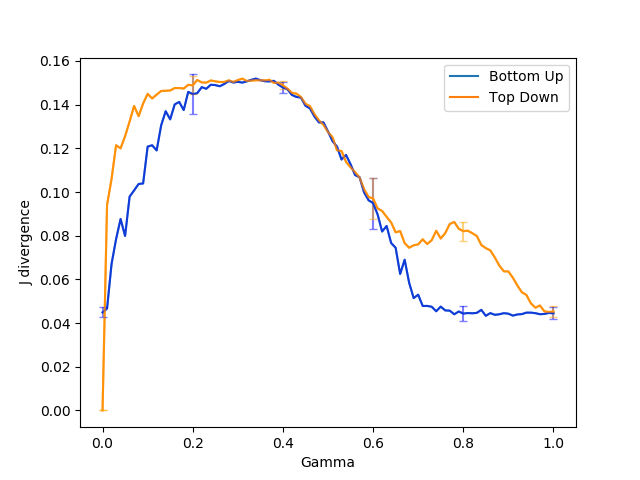
\includegraphics[width=\textwidth]{Images/Figures/BU+TD/FIE/J-Div_better.png}
    \caption{J-Divergence}
 \end{subfigure}
 %\hfill
 \begin{subfigure}[ht]{0.45\textwidth}
    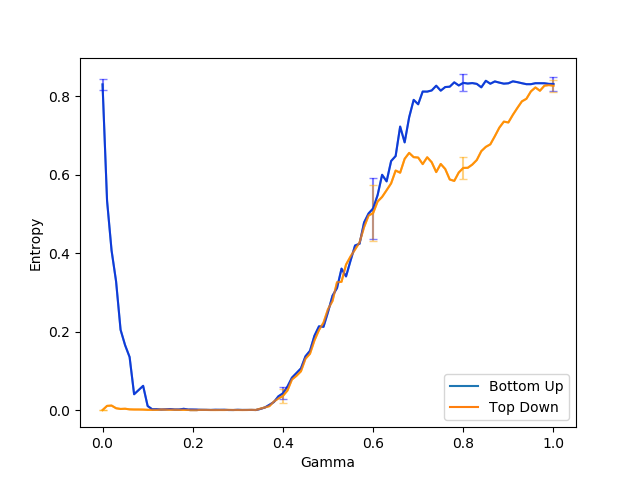
\includegraphics[width=\textwidth]{Images/Figures/BU+TD/FIE/Entropy_better.png}
    \caption{Entropy}
 \end{subfigure}

 \caption{Three plots showing the convergent behaviour of the Bottom Up and Top Down models with Discerning listeners as $\gamma$ is varied. (a) shows the time to convergence as defined by~\cref{eq:convergence}. (b) shows the average J-Divergence of the system at the corresponding iteration of (a). (c) shows the average entropy of the system at the corresponding iteration of (a). If the system has not converged within $50,000$ iterations, the point is left blank.} \label{fig:convergence_FIE}
\end{figure}



Here, the models converge at approximately the same rate for $ 0 \leq \gamma \leq 0.6$. However, it can be seen that the J-Divergence follows a parabola for this range of parameter values. This shows that the population is divided. As soon as the agents have the ability to ignore information their peers present, they form local consensuses. This manifests as groups of agents in different corners of the simplex, unable to accept an argument that comes from an agent in a different corner. As $\gamma$ increases, this division lessens, with agents becoming more able to hear other points of view. As $\gamma$ increases above $0.6$, the Bottom Up model begins to converge much more rapidly, as in the previous example. This is due to the harshness of the restriction placed on the speakers for high values of $\gamma$. As for high values of $\gamma$, the speaker must hold an extreme belief in a single state to be able to assert anything other than $\emptyset$. \Cref{fig:convergence_FIE} shows that both models converge at $4,000$ on average, significantly less than with Passive listeners. This is due to the local consensuses. The agents divide into small groups with low entropy values that change little over time, and so convergence is recorded without having to persuade the entire population to believe in a single state.  

The primary difference that emerges between these two models appears after $\gamma = 0.6$, where both entropy and J-Divergence plateau momentarily in the Top Down model. The difference is slight, and it is unclear exactly why it occurs. It is possible that this occurs because the Top Down model produces patterns such as those shown in~\cref{fig:sierpinski_triangle_intro}. The plateau indicates that these patterns are more stable than those formed by the Bottom Up model. At high values of $\gamma$, the Top Down model is likely to assert more general statements, and the listeners are more likely to accept them, leading to a more disparate and uncertain population than for the Bottom Up agents.

These results show that, when the listeners are capable of disregarding the assertions of a speaker, the population divides, forming local consensuses. Furthermore, the Top Down model is a slightly more robust solution for a wider range of $\gamma$. This is likely due to the greater level of flexibility built into the model. 



Now consider the convergence when the population comprised of Backfiring listeners. 


\begin{figure}
 \centering
  \begin{subfigure}[ht]{0.45\textwidth}
    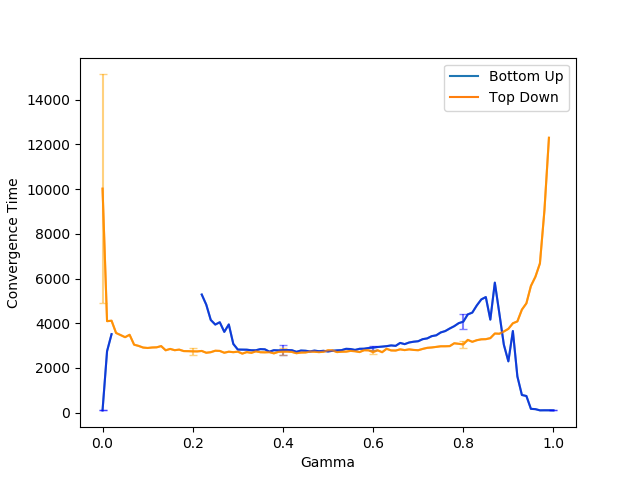
\includegraphics[width=\textwidth]{Images/Figures/BU+TD/Spiteful/Convergence.png}
    \caption{Convergence}
 \end{subfigure}
 \hfill
 \begin{subfigure}[ht]{0.45\textwidth}
    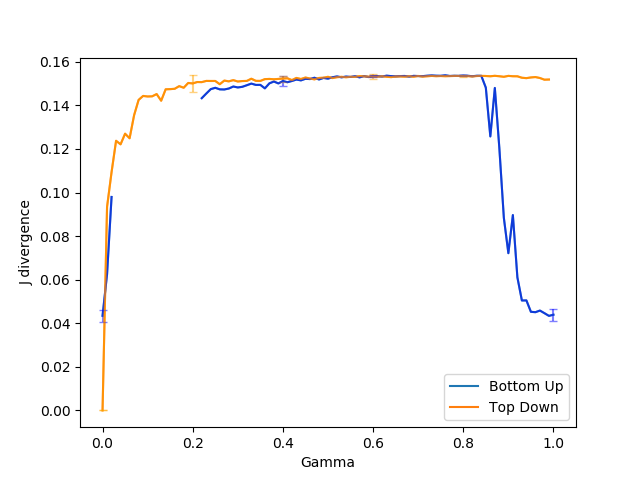
\includegraphics[width=\textwidth]{Images/Figures/BU+TD/Spiteful/J-Div.png}
    \caption{J-Divergence}
 \end{subfigure}
 \hfill
 \begin{subfigure}[ht]{0.45\textwidth}
    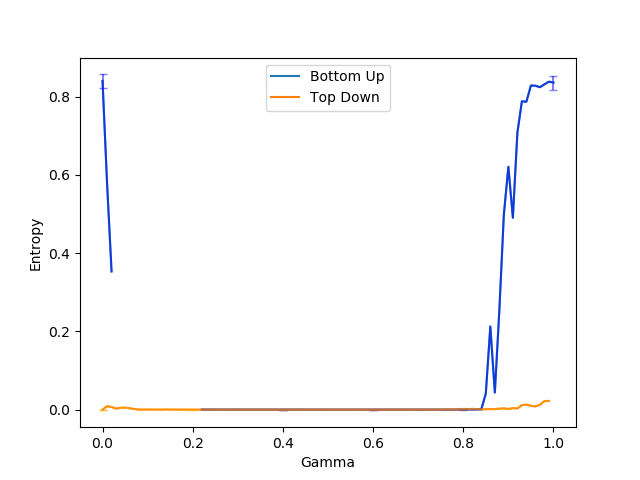
\includegraphics[width=\textwidth]{Images/Figures/BU+TD/Spiteful/Entropy.png}
    \caption{Entropy}
 \end{subfigure}
 \caption{Three plots showing the convergent behaviour of the Bottom Up and Top Down models with Backfiring listeners as $\gamma$ is varied. (a) shows the time to convergence as defined by~\cref{eq:convergence}. (b) shows the average J-Divergence of the system at the corresponding iteration of (a). (c) shows the average entropy of the system at the corresponding iteration of (a). If the system has not converged within $50,000$ iterations, the point is left blank.}\label{fig:convergence_Spite}
\end{figure}


It is clear from~\cref{fig:convergence_Spite} that the Bottom Up model fails to converge for $0.05 \leq \gamma \leq 0.2$. This is likely due to the general nature of a Bottom Up agent's assertions at these low values of $\gamma$. If the listener finds any one of the asserted states to be sufficiently improbable, they update on the complement of the asserted state, so general statements are less likely to meet this requirement than singletons.

It is apparent from the low value of entropy and high value of J-Divergence that the agents again reach local consensuses; they form distinct groups on the vertices of the simplex and are unable to listen to opposing arguments. Interestingly, the introduction of Backfiring listeners appears to have reduced the average convergence time compared to~\cref{fig:convergence_FIE} by $1,000$ iterations, a factor of $0.78$. This is likely due to the fact that, with Backfiring listeners, an agent updates at every iteration. The increased polarisation of updating on $\mathbf{A}^c$ will also contribute to an initial rapid division in the population. 


Finally, let us consider an Acclimatising population. Here, the population places less and less importance on new information as they receive each new argument. This promotes the stagnation of beliefs. \Cref{fig:convergence_Ageing} shows the convergence plots. 


\begin{figure}
 \centering
  \begin{subfigure}[ht]{0.45\textwidth}
    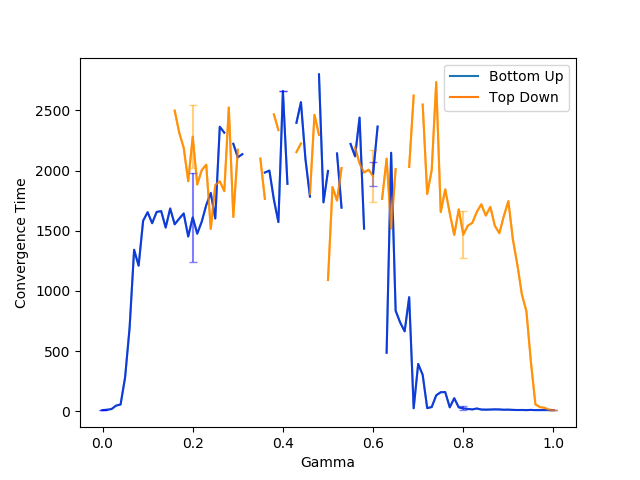
\includegraphics[width=\textwidth]{Images/Figures/ListenerModelPlots/Ageing/AgeingConvergenceDONTDELETE.png}
    \caption{Convergence}
 \end{subfigure}
 \hfill
 \begin{subfigure}[ht]{0.45\textwidth}
    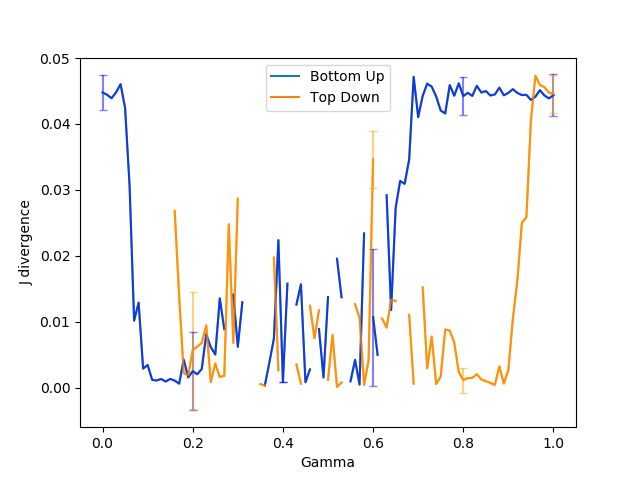
\includegraphics[width=\textwidth]{Images/Figures/ListenerModelPlots/Ageing/AgeingJ-DivDONTDELETE.png}
    \caption{J-Divergence}
 \end{subfigure}
 \hfill
 \begin{subfigure}[ht]{0.45\textwidth}
    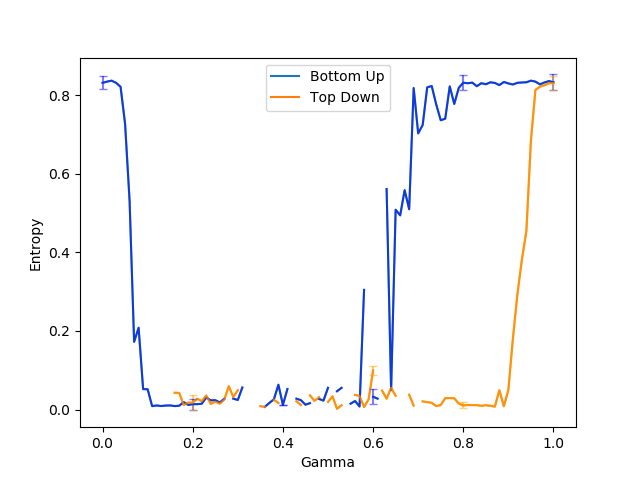
\includegraphics[width=\textwidth]{Images/Figures/ListenerModelPlots/Ageing/AgeingEntropyDONTDELETE(copy).png}
    \caption{Entropy}
 \end{subfigure}
 \caption{Three plots showing the convergent behaviour of the Bottom Up and Top Down models with Acclimatising listeners as $\gamma$ is varied. (a) shows the time to convergence as defined by~\cref{eq:convergence}. (b) shows the average J-Divergence of the system at the corresponding iteration of (a). (c) shows the average entropy of the system at the corresponding iteration of (a). If the system has not converged within $50,000$ iterations, the point is left blank.}\label{fig:convergence_Ageing}
\end{figure}


The results of these simulations are significantly more noisy than the other listener models. This is attributed to a number of factors. Firstly, this model converges within at most $2,500$ iterations, less than a third of the time taken by the Passive listener model, as one might expect. However, this rapid convergence both increases the appearance noise, by reducing the scale of the $y$-axis as well as increases the likelihood of variation in the results. When the simulation converges in so few iterations, minor anomalies in the order and nature of the arguments made in the population cause significant variation in the convergent behaviour of the system. For instance, consider an agent undecided between two possible states $H_1, H_2$, between which the remainder of the population is split evenly. If the individual agent repeatedly receives an argument in favour of $H_1$, it will update toward it, changing the entropy of the system. Whereas, if it receives alternating arguments, they will cancel out, registering as convergence. This leads to increased variation in the convergence times, dictated by the proportion of the population that is split between multiple states.

Despite this noise, observations can still be made. The convergence time under the Acclimatisation model is approximately one third less any other model, as one might expect. The agents update less and less upon hearing new information and so the rate of change in entropy decreases. For both speaker models, it can be seen that the entropy level is low for intermediate values of $\gamma$, with the Bottom Up model experiencing the same problem creating an argument is described in previous sections as $\gamma$ increases. The J-Divergence demonstrates a feature that has not previously been seen. While highly noisy, this plot shows that it is common to have non-zero J-Divergence using this model. Therefore, it must be the case that agents are spread out. However, in this model, this occurs in the following way. 

Consider a population with two local consensuses, where the population split approximately evenly between two states, as above. An agent that is undecided between the two will lie on the edge of the simplex. It will receive arguments from both subsets of the population, only increasing $\tau$, making the agent more stubborn. This agent will remain caught between the two groups until the system is said to have converged. The two main groups of agents will reinforce their current beliefs by communicating with other agents within the local consensus. This division in the population does not arise consistently, hence the noise in the J-Divergence plots. 


The Acclimatisation model shows similar behaviour for both the Bottom Up and Top Down models, both mostly achieving a population of agents certain in one state. However, this model occasionally divides the population. The main advantages of this model are the rapid convergence, and the ability for agents to grow wise with time. 





The results presented in this analysis demonstrate that when agents openly express the exact nature of their beliefs, the population becomes unanimously uncertain. However, when agents express arguments as sets of possible states of the world, it becomes possible for the population to form a global consensus in a single state, provided the listener agents are Passive. All the plots in this section demonstrate similarities between the Bottom Up and Top Down models for intermediate values of $\gamma$. However, for extremely high values, the Bottom Up model fails to produce meaningful assertions. The Top Down model is more robust, with slow convergence times occurring for very low values of $\gamma$. The two behave similarly, although Top Down model is a more robust approach for a wider range of values for $\gamma$. Furthermore, the Optimised model is shown to be incapable of reliably producing a consensus in a single state of the world, highlighting that its unconstrained approach is disadvantageous for the population. 

When listeners are able to discriminate, rejecting information that they deem unlikely, the population polarises. Local consensuses form, with subsets of the population unable to communicate with each other. This results in more rapid convergence, though not to a single state of the world. Finally, agents in the Acclimatising model converge more rapidly than any other model, though unpredictably lead to divisions in the population, again forming local consensuses. The only models that regularly give rise to global consensus in a single belief are the Top Down and Bottom Up models with Passive listeners, with the Top Down model behaving consistently across the full range of $\gamma$. 

\chapter{Extensions}

\section{The Introduction of Evidence} \label{sect:evidence}

In many studies of multi-agent communication, there exists a ``true state'' of the world that the agents must agree upon. Here, we will explore the effects of including such a state as well as evidence in support of it. We arbitrarily assign one state of the world to be ``true''. At each iteration, a subset of the population is selected to receive evidence. This is done by conducting $K$ Bernoulli trials, with probability $\pi$. There is also a chance $c$ that the evidence is accurate. This can be thought of as an agent querying an external, fallible oracle. Here, the oracle returns a singleton set, containing a single element that is only partially accurate. This assertion is then incorporated into the agent's beliefs as in~\cref{eq:BU_update_rule}

It is expected that the introduction of this evidence will sway the agents towards the true state of the world when $c > \frac{1}{n}, \pi > 0$, an expectation supported by~\cref{fig:evidence}. In this figure, the true state of the world is rotated on the $2,000^{\textnormal{th}},5,000^{\textnormal{th}},10,000^{\textnormal{th}} $ and $ 20,000^{\textnormal{th}}$ iterations. \cref{fig:evidence_deviation} shows the average J-Divergence between the true state of the world and each agent at each time step, referred to as the deviation. 


\begin{figure}[H]
 \centering
  \begin{subfigure}[ht]{0.45\textwidth}
    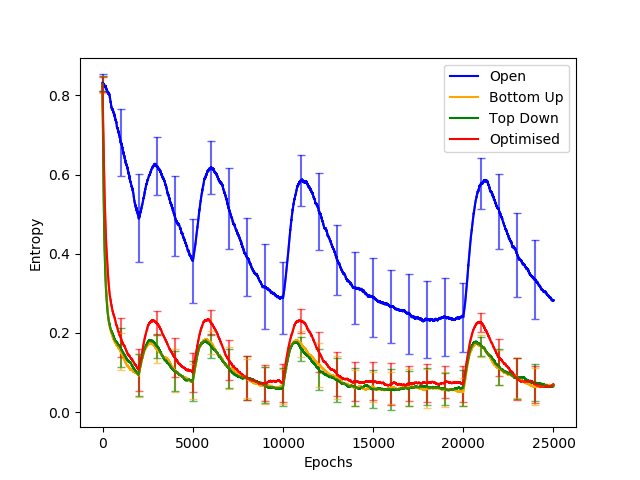
\includegraphics[width=\textwidth]{Images/Figures/Evidence/EntropyGood.png}
    \caption{Entropy}
 \end{subfigure}
 \hfill
 \begin{subfigure}[ht]{0.45\textwidth}
    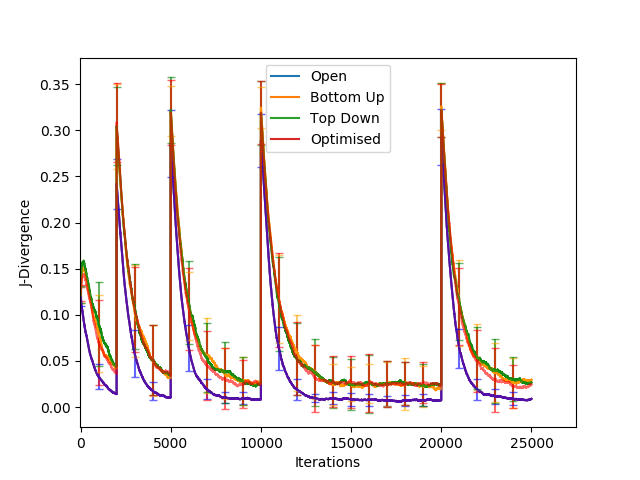
\includegraphics[width=\textwidth]{Images/Figures/Evidence/J-DivGood.png}
    \caption{Deviation} \label{fig:evidence_deviation}
 \end{subfigure}
 \caption{Two plots to show the change in entropy and deviation from the true state over time, for the Open, Bottom Up, Top Down, and Optimised models. These plots were obtained using Passive listeners, and were averaged over $100$ runs. Here, $\pi = 0.001, c=0.9$. At the $2,000^{\textnormal{th}},5,000^{\textnormal{th}},10,000^{\textnormal{th}} $ and $ 20,000^{\textnormal{th}} $, the true state of the world $H_j$ is switched to be $H_{j+1}$, highlighted by the jumps in deviation between the true state and each agent.}\label{fig:evidence}
\end{figure}

It can be clearly seen that the entropy in the Open model is significantly higher than the rest of the models. Recalling the results of~\cref{sect:analysis}, this is not unexpected. The agents in the Open model cluster together, forming a group in the centre of the simplex. With probability $\pi$, an agent is selected to receive evidence, therefore leaving the main group. Each time such an agent is selected as speaker while outside the group, the centroid of the population moves toward it. When both $\pi$ and $c$ are sufficiently large, this moves the entire population toward the true state. It is apparent that the Open model has the smallest deviation of any of the models, as shown in~\cref{fig:evidence_deviation}. The other three models behave similarly in these plots. At first sight, this does not seem to make sense in conjunction with the highest entropy value on the plot. However, agents in the other three models have a tendency to lie along the edges of the simplex, for which entropy values are low, whereas the Open model rarely reaches these extremities. Instead, agents in the Open model move cohesively in the direction of the true state, getting all the agents close, yielding a small deviation. Conversely, the other models achieve large numbers of agents with strong beliefs in a subset of the possible worlds, that are not as close to the true state as the Open model. 

Another factor in favour of the Open model in this paradigm is that the magnitude of its updates is much smaller than the other models. Consider an agent $x$, such that $\underline{\mathbf{P}}^t_x = [0.4, 0.6, 0]^T$. This agent is undecided between two states, with a slight preference for $H_2$. In this example, let the rest of the population be almost certain in the true state, $H_1$. If $x$ is selected as speaker in the Bottom Up, Top Down, or Optimised model, it is likely that it will assert $\mathbf{A} = \{ H_2 \}$. In this case, the listener agent will update $\approx \alpha$ toward $H_2$, as in~\cref{fig:sierpinski_triangle_intro}. However, if $x$ is an Open agent, it broadcasts its beliefs, causing the listener to update only $\approx \frac{\alpha}{2}$ towards $H_2$. This means that the Open model is slightly slower to react, but much more robust to changes, inexorably updating towards the true state.  

When the true state of the world is rotated, all models recover, with the agents quickly re-converging to the true state. This change in the true state corresponds with the vertical sections of~\cref{fig:evidence_deviation}. This recovery is only possible for agents that have not reached certainty in a single state. Once an agents beliefs $\underline{\mathbf{P}}_x^t = [1,0,0]^T$ it is impossible to persuade them to alter their opinions. In simulation, this the true state to remain the same for many thousands of iterations, depending on $\pi$ and $c$. 


\section{Method for the Reconstruction of an Agent's Beliefs}

In this Optimised model, it is assumed that the agents have access to perfect information about the nature of the listener's beliefs before they make an assertion. In this model, the speaker creates the argument that will cause the listener to update their beliefs to be as close as possible to the speaker. The complete understanding of the way in which the listener will react is highly unrealistic, as it is rare that any agent would be so open or predictable. To weaken this assumption it is possible to reconstruct the listener's beliefs based on their previous assertions as speaker.

Let each agent in the population keep a record of the last $\zeta$ assertions that each speaker has made in the set $\mathbf{A}_\zeta$. It is likely that the average of these assertions will reflect an agent's underlying set of beliefs. Hence, the speaker takes an average of the last $\zeta$ assertions by the listener to approximate their beliefs at the current time step, re-normalising it to be a probability distribution. This approximation takes the form

\begin{equation} \label{eq:reconstructive}
    \hat{p}_{l,j} = \frac{\abs{ \{H_j: H_j \in \mathbf{A}_\zeta \} } }{ \sum_k^n \abs{ \{ H_k; H_k \in \mathbf{A}_\zeta \} }   }
\end{equation}

\Cref{fig:reconstructive} shows a comparison between the standard Optimised model with perfect information and with reconstructed information. 


\begin{figure}[H]
 \centering
  \begin{subfigure}[ht]{0.45\textwidth}
    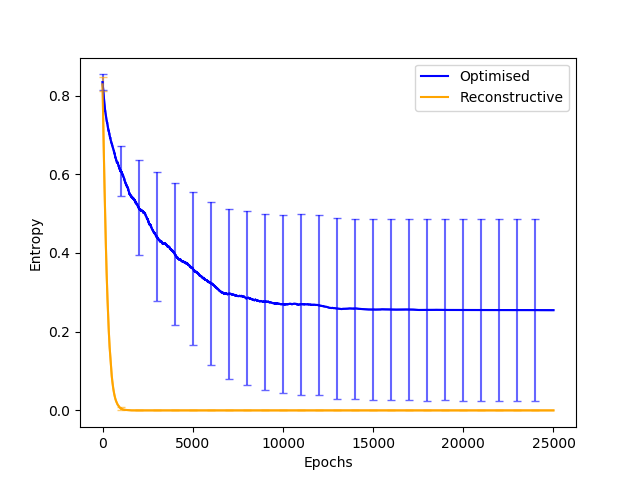
\includegraphics[width=\textwidth]{Images/Figures/Reconstructive/Entropy_reconstruct_better.png}
    \caption{Entropy}
 \end{subfigure}
 \hfill
 \begin{subfigure}[ht]{0.45\textwidth}
    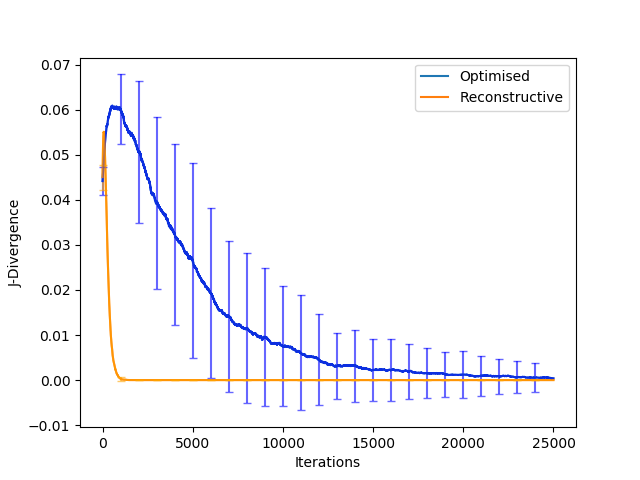
\includegraphics[width=\textwidth]{Images/Figures/Reconstructive/J-Div_reconstruct_better.png}
    \caption{J-Divergence}
 \end{subfigure}
 \caption{Two plots to show the change in entropy and J-Divergence over time, for the Optimised model with perfect information and reconstructed information at $\zeta = 10$. These plots were obtained using Passive listeners, and were averaged over $100$ runs.}\label{fig:reconstructive}
\end{figure}

This shows that the reconstructive model almost immediately achieves a consensus in a single state of the world. This behaviour is highly consistent, as shown by the narrow error bars. However, the Optimised model with perfect information again underperforms. The J-Divergence decreases to $0$ suggesting that the agents do reach a consensus, however, the consensus appears to be in an uncertain distribution. It is likely that the width of the error bars in the entropy plot is due to the Optimised model again converging to a vertex in one of the sub-triangles of~\cref{fig:chaos_game}. 

It is interesting to note that the error between the listener's beliefs and the speaker's approximation decreases to $0$. This is intuitive, as once an agent is highly confident in a single state, it will likely assert that single state alone. Thus the approximation will become based on the repeated assertion of a single state, decreasing to $0$ as the system converges. 

These results show that the Optimised model is an insufficient method for achieving consensus with perfect information, however, with approximate information, it quickly converges to a certain consensus. 



\section{Mixed Populations Tests} \label{sect:pop_tests}

In Economics, agents can be assigned a variety of different trading strategies, with the aim of making deals that maximise the agent's profit. The earliest strategies proposed were rudimentary, such as ZI-U and ZI-C~\cite{Gode1993AllocativeRationality}, with later models incorporating machine learning techniques to improve their performance, such as ZI-P, GDX and AA~\cite{Cliff1997Minimal-IntelligenceEnvironments, Gjerstad1998PriceAuctions, Vytelingum2006TheAuction}. \cite{Vach2015ComparisonAgents} provides an excellent comparison of the performance of these strategies when tested against each other in various concentrations. This analysis inspires the following analysis. In order to determine the most persuasive argumentation strategy, two different speaker models can be included in the same population. A record is kept of the change in J-Divergence that is attributed to arguments created by both models, and the ``victor'' is the model that accounts for the greatest change in J-Divergence after $5,000$ iterations. Furthermore, different concentrations of each strategy should be considered, as, in Vach's work, some strategies perform best when in a minority. 

The following table shows the mean and standard deviation of the J-Divergence, summed for the model of each speaker across $5,000$ iterations for a population of $100$ agents mixed to the corresponding concentrations. It also shows the fraction of those $1,000$ runs that was ``won'' by each strategy. The victors are shown in bold. It is important to note that these experiments assume each interaction between a speaker and listener to be independent, such that the order in which agents attempt to persuade each other is unimportant. This is the ``well-stirred'' assumption~\cite{Parker2009CooperativeProblem}. 

\begin{table}[H]
\begin{adjustbox}{max width = \textwidth}
\begin{tabular}{ll||cc|cc|cc|cc|cc|cc}
 &  & Open & Bottom Up & Open & Top Down & Open & Optimised & Bottom Up & Top Down & Bottom Up & Optimised & Top Down & Optimised \\ \hline \hline
\multirow{3}{*}{1:5} & Wins & 0 & \textbf{1000} & 0 & \textbf{1000} & 0 & \textbf{1000} & 0 & \textbf{1000} & 0 & \textbf{1000} & 0 & \textbf{1000} \\
 & Mean & 102.62 & 556.77 & 266.24 & 310.25 & 32.71 & 461.35 & 116.48 & 572.93 & 98.44 & 559.44 & 114.65 & 537.71 \\
 & Standard Deviation & 33.89 & 182.86 & 83.19 & 96.71 & 10.48 & 165.44 & 37.39 & 178.11 & 976.91 & 169.07 & 34.24 & 161.23 \\ \hline
\multirow{3}{*}{2:4} & Wins & 0 & \textbf{1000} & 0 & \textbf{1000} & 0 & \textbf{1000} & 0 & \textbf{1000} & 0 & \textbf{1000} & 0 & \textbf{1000} \\
 & Mean & 195.84 & 434.74 & 196.56 & 439.31 & 63.32 & 301.55 & 237.99 & 465.36 & 197.7 & 459.79 & 235.58 & 573.71 \\
 & Standard Deviation & 62.09 & 138.50 & 61.76 & 136.48 & 21.72 & 118.50 & 71.09 & 178.11 & 65.07 & 138.96 & 34.24 & 131.35 \\ \hline
\multirow{3}{*}{3:3} & Wins & 15 & \textbf{985} & 2 & \textbf{998} & 0 & \textbf{1000} & \textbf{763} & 237 & 0 & \textbf{1000} & 25 & \textbf{975} \\
 & Mean & 259.22 & 298.03 & 268.98 & 313.77 & 91.57 & 191.49 & 340.28 & 328.92 & 300.58 & 357.97 & 345.47 & 377.57 \\
 & Standard Deviation & 87.52 & 101.61 & 86.28 & 100.07 & 33.15 & 76.38 & 110.83 & 106.40 & 100.03 & 104.51 & 106.46 & 102.59 \\ \hline
\multirow{3}{*}{4:2} & Wins & \textbf{1000} & 0 & \textbf{1000} & 0 & \textbf{757} & 243 & \textbf{1000} & 0 & \textbf{997} & 3 & \textbf{1000} & 0 \\
 & Mean & 275.46 & 168.0 & 296.03 & 186.38 & 114.61 & 109.65 & 470.81 & 223.92 & 421.71 & 256.17 & 471.36 & 267.90 \\
 & Standard Deviation & 101.28 & 63.77 & 101.13 & 63.80 & 38.93 & 42.83 & 142.78 & 67.31 & 137.47 & 68.12 & 135.33 & 63.46 \\ \hline
\multirow{3}{*}{5:1} & Wins & \textbf{789} & 211 & \textbf{1000} & 0 & \textbf{1000} & 0 & \textbf{1000} & 0 & \textbf{1000} & 0 & \textbf{1000} & 0 \\
 & Mean & 261.47 & 256.25 & 242.22 & 76.76 & 125.61 & 50.62 & 571.24 & 109.50 & 541.02 & 139.20 & 585.96 & 143.79 \\
 & Standard Deviation & 87.74 & 97.96 & 89.27 & 29.16 & 40.51 & 19.65 & 181.24 & 33.52 & 178.71 & 33.59 & 171.96 & 31.57
\end{tabular}
\end{adjustbox}
\caption{Table to show results of mixing different persuasion strategies together in different concentrations, with Passive listeners. The victor of the majority of the $1,000$ games is shown in bold, alongside the mean and standard deviation J-Divergence each strategy is responsible for. }
\end{table}


The results of this experiment are much as one would expect, showing that, in almost all cases, the agent in the majority is responsible for the most movement in the population. However, there are some cases where a strategy underperforms. For instance, the Open vs Optimised games with a $4:2$ concentration show the Optimised solution winning $24.3 \%$ of the time. This highlights the limitations of the Open model, as demonstrated in~\cref{sect:evidence}, with its more diluted arguments limiting the potency of the argument. Another remarkable observation is the result of the Open vs Bottom Up game with a $5:1$ concentration. This is unexpected and the reasons for it are unclear. It is unlikely to be anomalous as the system was run for $1,000$ games. It is possible that testing other similar concentrations might reveal a trend, though, at present, none is apparent.

It can also be seen that the Optimised model appears to dominate the balanced group tests at concentrations $3:3$, only losing $25$ games to the Top Down model. This suggests that its ability to assert anything it must to change the listener's beliefs causes a large amount of movement in the population, at least during the first $5,000$ iterations. The same $3:3$ tests also show minor differences between the Bottom Up and Top Down models. When competing directly, the Bottom Up strategy appears to be more persuasive, winning the $3:3$ contests by a clear margin, though their mean movement is similar when performing in the same concentrations. For instance, in the $1:5$ test, the Top Down model caused approximately the same degree of movement as the Bottom Up caused in the $1:5$. 

\chapter{Conclusions}

While previous protocols for the combination of beliefs in multi-agent systems have produced effective tools for reaching a global consensus in the population, they are unrefined, with agents communicating the exact nature of their beliefs. The models in~\cref{sect:speaker_models} demonstrate a variety of different convergent behaviours. It has been demonstrated both analytically and numerically that the populations of Bottom Up and Top Down agents converge to a consensus in a single state of the world, when the listeners are Passive. These models behave similarly, though the Top Down model produces more consistent convergent behaviour as $\gamma$ is varied. The introduction of listeners capable of disregarding information they deem unlikely divides the population. Local consensuses form in opposing, single states of the world, with listeners unable to accept an argument from an agent they do not already agree with. 

The Open and Optimised models are impractical for the purposes of achieving a global consensus. Though the population does form a consensus, it is not in any one state of the world. Instead, the agents cluster together no more confident in one state than another. The Optimised approach is impractical for two reasons. Firstly, the assumption of perfect information is unlikely to be realistic. Secondly, populations of agents practising the Optimised approach regularly converge to uncertain beliefs and remain there. This is a result of their unwillingness to make an assertion that will persuade the listener to update to be further away from the speaker. Interestingly, when the Optimised model uses reconstructed information, it rapidly converges to a practical consensus. Furthermore, the persuasive power demonstrated by the Optimised Model in~\cref{sect:pop_tests} highlights the dangers of ``dark side'' technologies. 

When agents have the power to disregard information they deem unlikely, populations of Bottom Up or Top Down agents no longer reliably form a global consensus. The ability to ignore incredible information polarises the population, forming distinct local consensuses that are unable to communicate with agents that they do not already agree with. This does lead to more rapid convergence than simply using Passive listeners, but fails to create consensus in a single state. Finally, when the Bottom Up and Top Down models are applied to Acclimatising listeners, the convergence is even more rapid as agents quickly become unwilling to alter their beliefs, no matter how persuasive the argument may be. Similar to the Optimised model, this can lead to consensus in a single state, but regularly only achieves local consensus, often with agents few agents uncertain between two conflicting states, uncertain of which to believe. 

All the models in this research show aptitude for different tasks. The Open model is the quickest to converge and the most robust to adapt to evidence it receives though it does not reach certainty in a single state. The Bottom Up model causes a slightly greater affective change than the Top Down approach, however, the Top Down approach is a more robust model, functioning well for a wide variety of parameters. Finally, the Optimised model is powerful though impractical, converging quickly though failing to produce a global consensus in a single possible state of the world. 


\section{Further Work}

The analysis in~\cref{sect:analysis} explores the effects of varying a single parameter $\gamma$. However, it would be interesting to explore the impact of varying both $\gamma$ and $\alpha$ simultaneously. This might highlight the particularly strong performance of models when parameter values are at their most extreme.

Similar to the Acclimatisation model, further functions for the value of $\alpha$ could demonstrate interesting behaviour. For instance, if $\alpha$ was given by the cosine similarity between the assertion and the listeners beliefs, or, as in~\cite{Hegselmann2002OpinionSimulation}, the listener's perceived reliability of the speaker. 

Further work could also be conducted incorporating aspects of the Peripheral Route of the ELM, such as the mood of the listener, or the fact that, when an agent feels they are being persuaded, they are harder to convince. Alternatively, strategies in which the speaker targeted particularly influential listeners could be explored, potentially applying elements of Machine Learning to do so.

This research area is young and full of potential, therefore there are likely many further avenues worth investigating. These are but a few. 



\newpage
\bibliographystyle{apalike}
\bibliography{references.bib}

\end{document}